\section{Implementation with the ROS framework}

\subsection{Introduction to the ROS framework}

\textbf{ROS} is an open-source robotics software framework. It is a meta-operating system, which means that it provides its own 
abstractions on top of the host's operating system including filesystem, hardware abstractions, low-level device control, 
package management and networking. It also provides tools and services to develop large, scalable 
robotics software, it supports a wide variety of libraries and programming languages and it has a huge community, support and 
documentation resources.

\begin{center}
\begin{figure}[H]
\centering
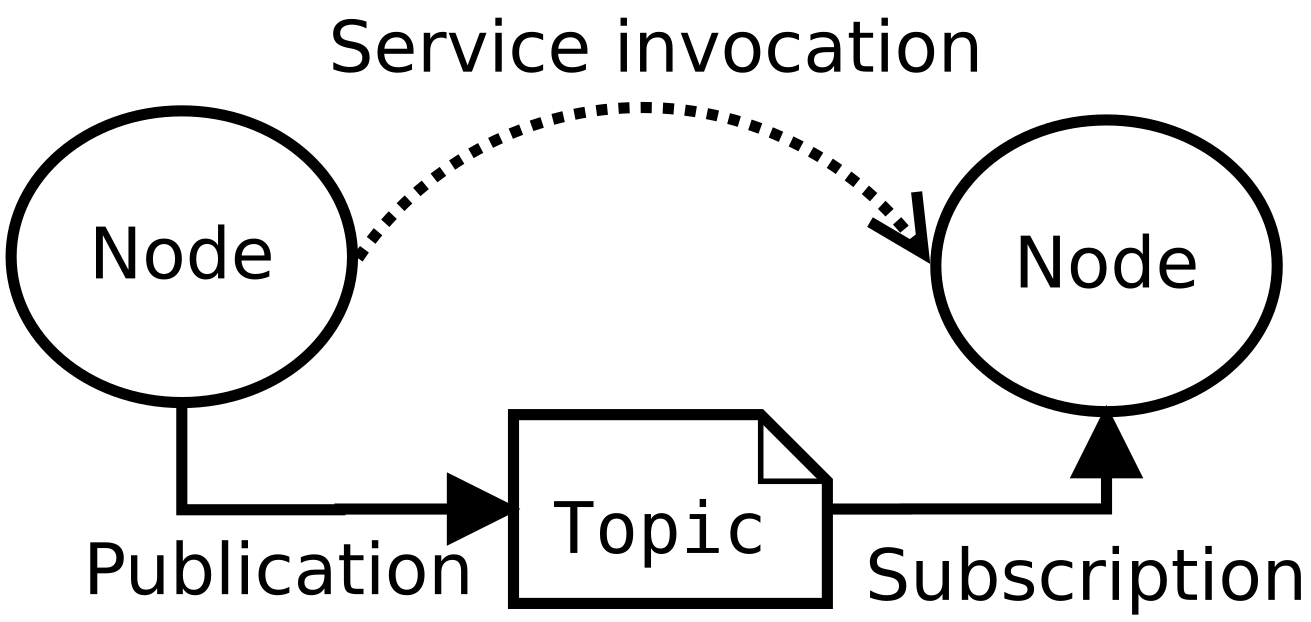
\includegraphics{images/ROS_basic_concepts_topics_nodes.png}\\
\caption{Communication diagram of 2 ROS nodes with a topic and a service}
\end{figure}
\end{center}


\subsection{Gazebo simulation environment}

\begin{center}
\begin{figure}[H]
\centering
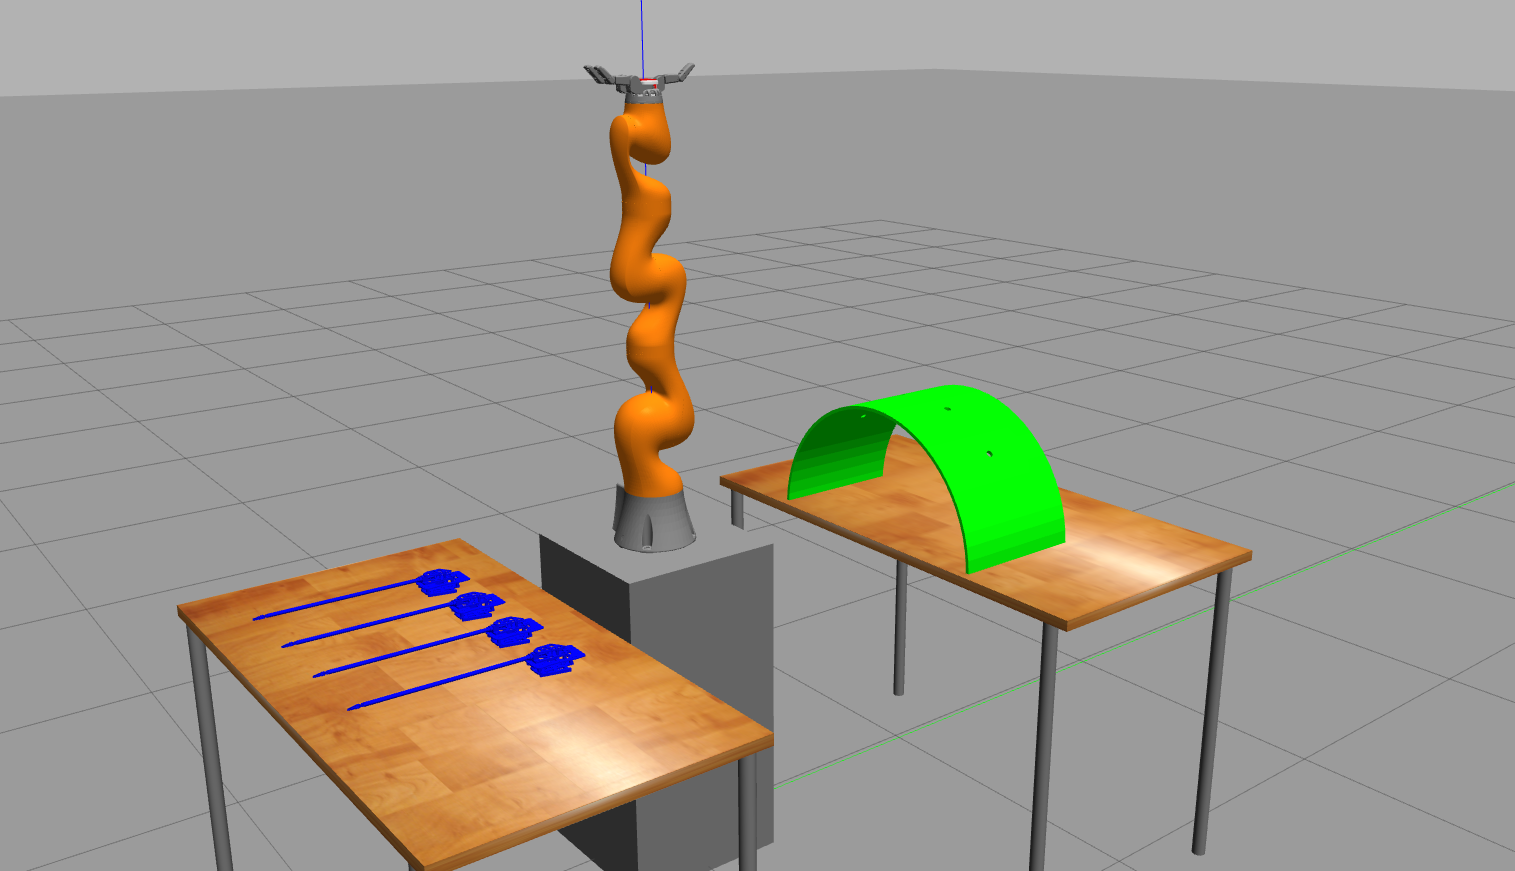
\includegraphics[width=12cm]{images/gazebo-sim1.png}\\
\caption{Simulation environment in Gazebo}
\end{figure}
\end{center}

The main environment setup of this thesis was designed using the Gazebo simulation environment and 
it consists of the following objects:
\begin{itemize}
\item the robot arm, KUKA\textsuperscript \textregistered iiwa14 lbr, being at the center of the setup
\item the robot base, so that the robot arm can better reach the tools and the surgical site and have more flexibility in movement
\item 2 tables, one for the tools and one for the surgical site
\item 4 surgical tools, using a modified version of the surgical tools used in the Raven II surgical platform
\item a mounting dock, which has holes that have the same role as the trocars (small tubes from 
which the surgical tool is inserted). Initially a mounting dock with 4 same holes of 4mm diameter was used, but it was later replaced with a new one with holes of variable diameters to test feasibility of pivot motions. Larger diameters means more space for motion planner to search for solution and thus more probable to find a solution.
\end{itemize}

\begin{center}
\begin{figure}[H]
\centering
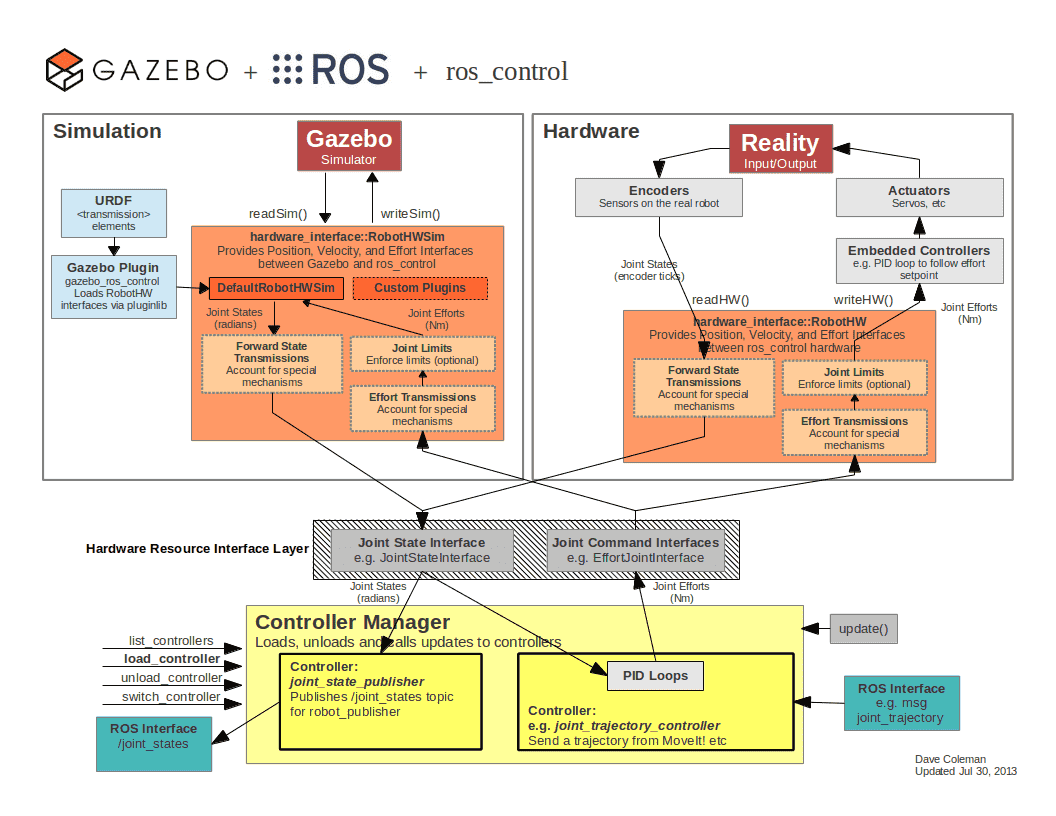
\includegraphics[width=12cm]{images/Gazebo_ros_transmission.png}\\
\caption{Control \& Hardware Interfaces in Gazebo and ROS}
\end{figure}
\end{center}


\subsection{Visualization with RViz}

RViz is one of the most important and most used tools in robotic applications development and is a 3D visualizer for the Robot Operating System framework. RViz functionality should not be confused 
with that of Gazebo, because the first one visualizes the robot state and the \textbf{perceived} world (perceived objects or other calculations related to the world) whereas the second one simulates the real world.

\begin{center}
\begin{figure}[H]
\centering
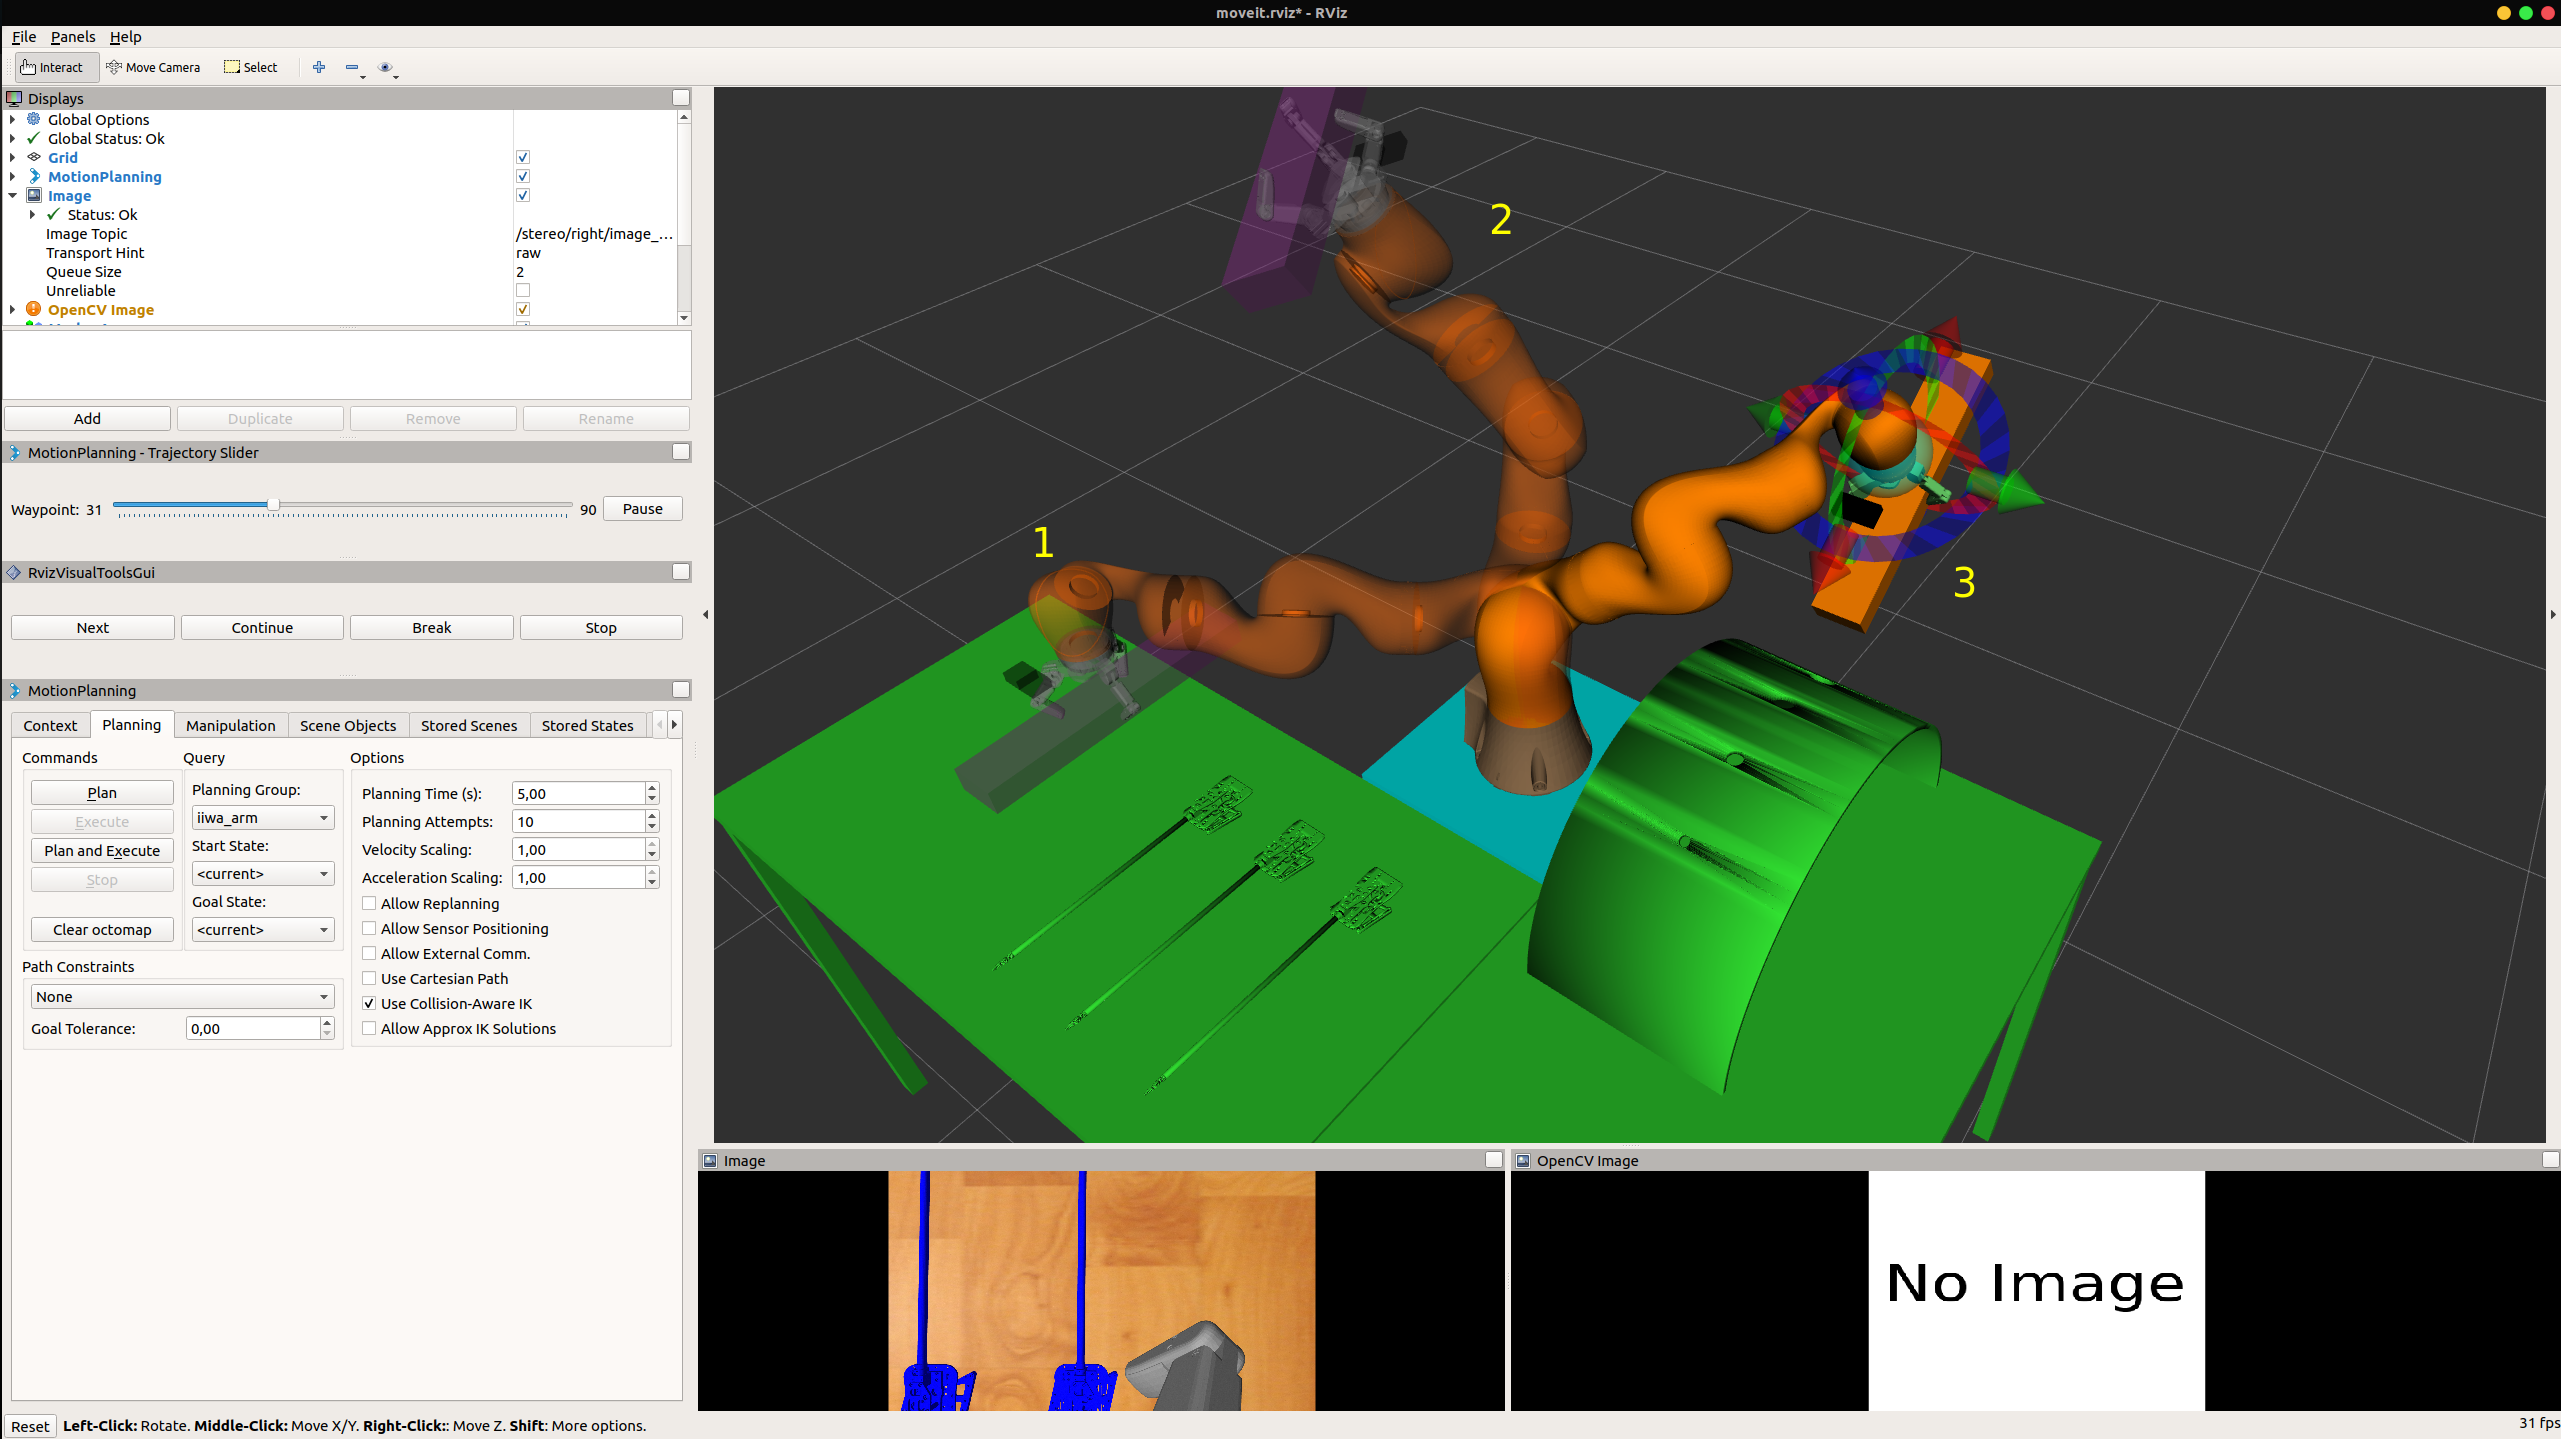
\includegraphics[width=\textwidth]{images/rviz.png}\\
\caption{RViz: Visualizing the robot state as well as the state of the perceived world\\
In this screenshot, various poses of the robot are shown: 1) the current actual real pose of the robot, 2) the planned pose and 3) the goal pose, which can 
freely be moved within the RViz environment}
\end{figure}
\end{center}

The objects that appear in RViz can either be visualized from approximations calculated from actual measurements from the robot (for example a point cloud) or can be manually loaded, in which case we make 
an assumption that the robot already "knows" the exact position, orientation, size and shape of the object, which is rarely the case in real life scenarios.
It is important to mention, that every such object is taken into consideration in collision checks and in path planning algorithms.

\subsection{Motion Planning with Moveit}

When using the Moveit ROS library a set of parameters need to be configured in order to generate the desired commands for the controller:
\begin{itemize}
	\item Position tolerance:
	\item Orientation tolerance:
	\item Maximum planning time:
	\item Replanning:
	\item Maximum planning attempts:
	\item Base frame:
	\item Jump threshold:
	\item Velocity scaling factor:
	\item End-effector step:
	\item Planner algorithm:
	\item Fraction:
\end{itemize}

Typical motion planning parameter values outside of surgical site:
\begin{itemize}
	\item Position tolerance: 50μm
	\item Orientation tolerance: 0.00005 deg
	\item Planning time: 10s
\end{itemize}

Typical motion planning parameter values inside surgical site:
\begin{itemize}
	\item Position tolerance:
	\item Orientation tolerance:
	\item Planning time
	\item End-effector interpolation step: 1mm
	\item Maximum velocity scaling factor
\end{itemize}

Sometimes the motion planner finds a solution but the execution from the controller is aborted. 
After many iterations of the same experiment this does not happen always, which means that the 
feasibility of the execution of the movement by the controller depends on the initial state of 
the robot, i.e. if initially some joints of the robot are at their boundaries, then the next 
commanded trajectory maybe unfeasible. Another reason that the path planner may fail is the 
probabilistic nature of the path planning algorithms (see also RRT and PRM algorithms in chapter 6).

At each time step it is important to publish a custom message containing all the information 
about the kinematic state of the robot. In this thesis a custom \textbf{ROS} message was created 
containing a tf transform with a 3D vector for the position and a quaternion for the rotation and 
a custom  6-by-7 matrix containing the values of the Jacobian. The MoveIt library, from which the 
kinematic state of the robot is obtained, returns the orientation of the end effector as a 3-by-3 
rotation matrix, but in the ROS tf message it must be expressed as a quaternion. To convert the 
matrix to a quaternion we first calculate the euler angles and then use these values to construct 
the quaternion “vector”. The quaternion representation of rotation is often preferred in robotic 
applications due to its efficiency in calculations and memory. To convert the transformation 
matrix to euler angles and then to quaternions the following formulas were used:
\[
T = 
\begin{bmatrix}
r_{11} & r_{12} & r_{13} & x \\
r_{21} & r_{22} & r_{23} & y \\
r_{31} & r_{32} & r_{33} & z \\
0 & 0 & 0 & 1\\
\end{bmatrix}
\]

\[
φ = atan2(r_{21}, r_{11})
\]

\[
θ = atan2(-r_{31}, \sqrt{r_{11}^2 + r_{21}^2})
\]

\[
ψ = atan2(r_{32}, r_{33})
\]

where $T$ is the transformation matrix and $φ, θ, ψ$ are the roll, pitch and yaw (Euler) angles.




\subsection{Experiments and Development methodology}

\subsubsection{Robot Planner 1}

In this first experiment we are testing some simple trajectories with the surgical tool already attached to the robot arm's end effector.
The path is designed using the appropriate coordinates and orientations so that the robot begins from the home position, then visits the table with the surgical 
tools and then visits the other table on top of which the mounting dock is placed. Upon arrival at the mounting dock, the robot inserts the tool inside a hole
(we consider these holes to be a simplistic alternative to the trocars used in real operations), then executes a simple pivot motion, while the tool is still 
inserted and then the tool gets ejected from the mounting dock's hole.\\

The aim of this experiment is to test the overall behaviour of the robot inside the work space, before implementing more complex path planning algorithms.

\begin{center}
\begin{figure}[H]
\centering
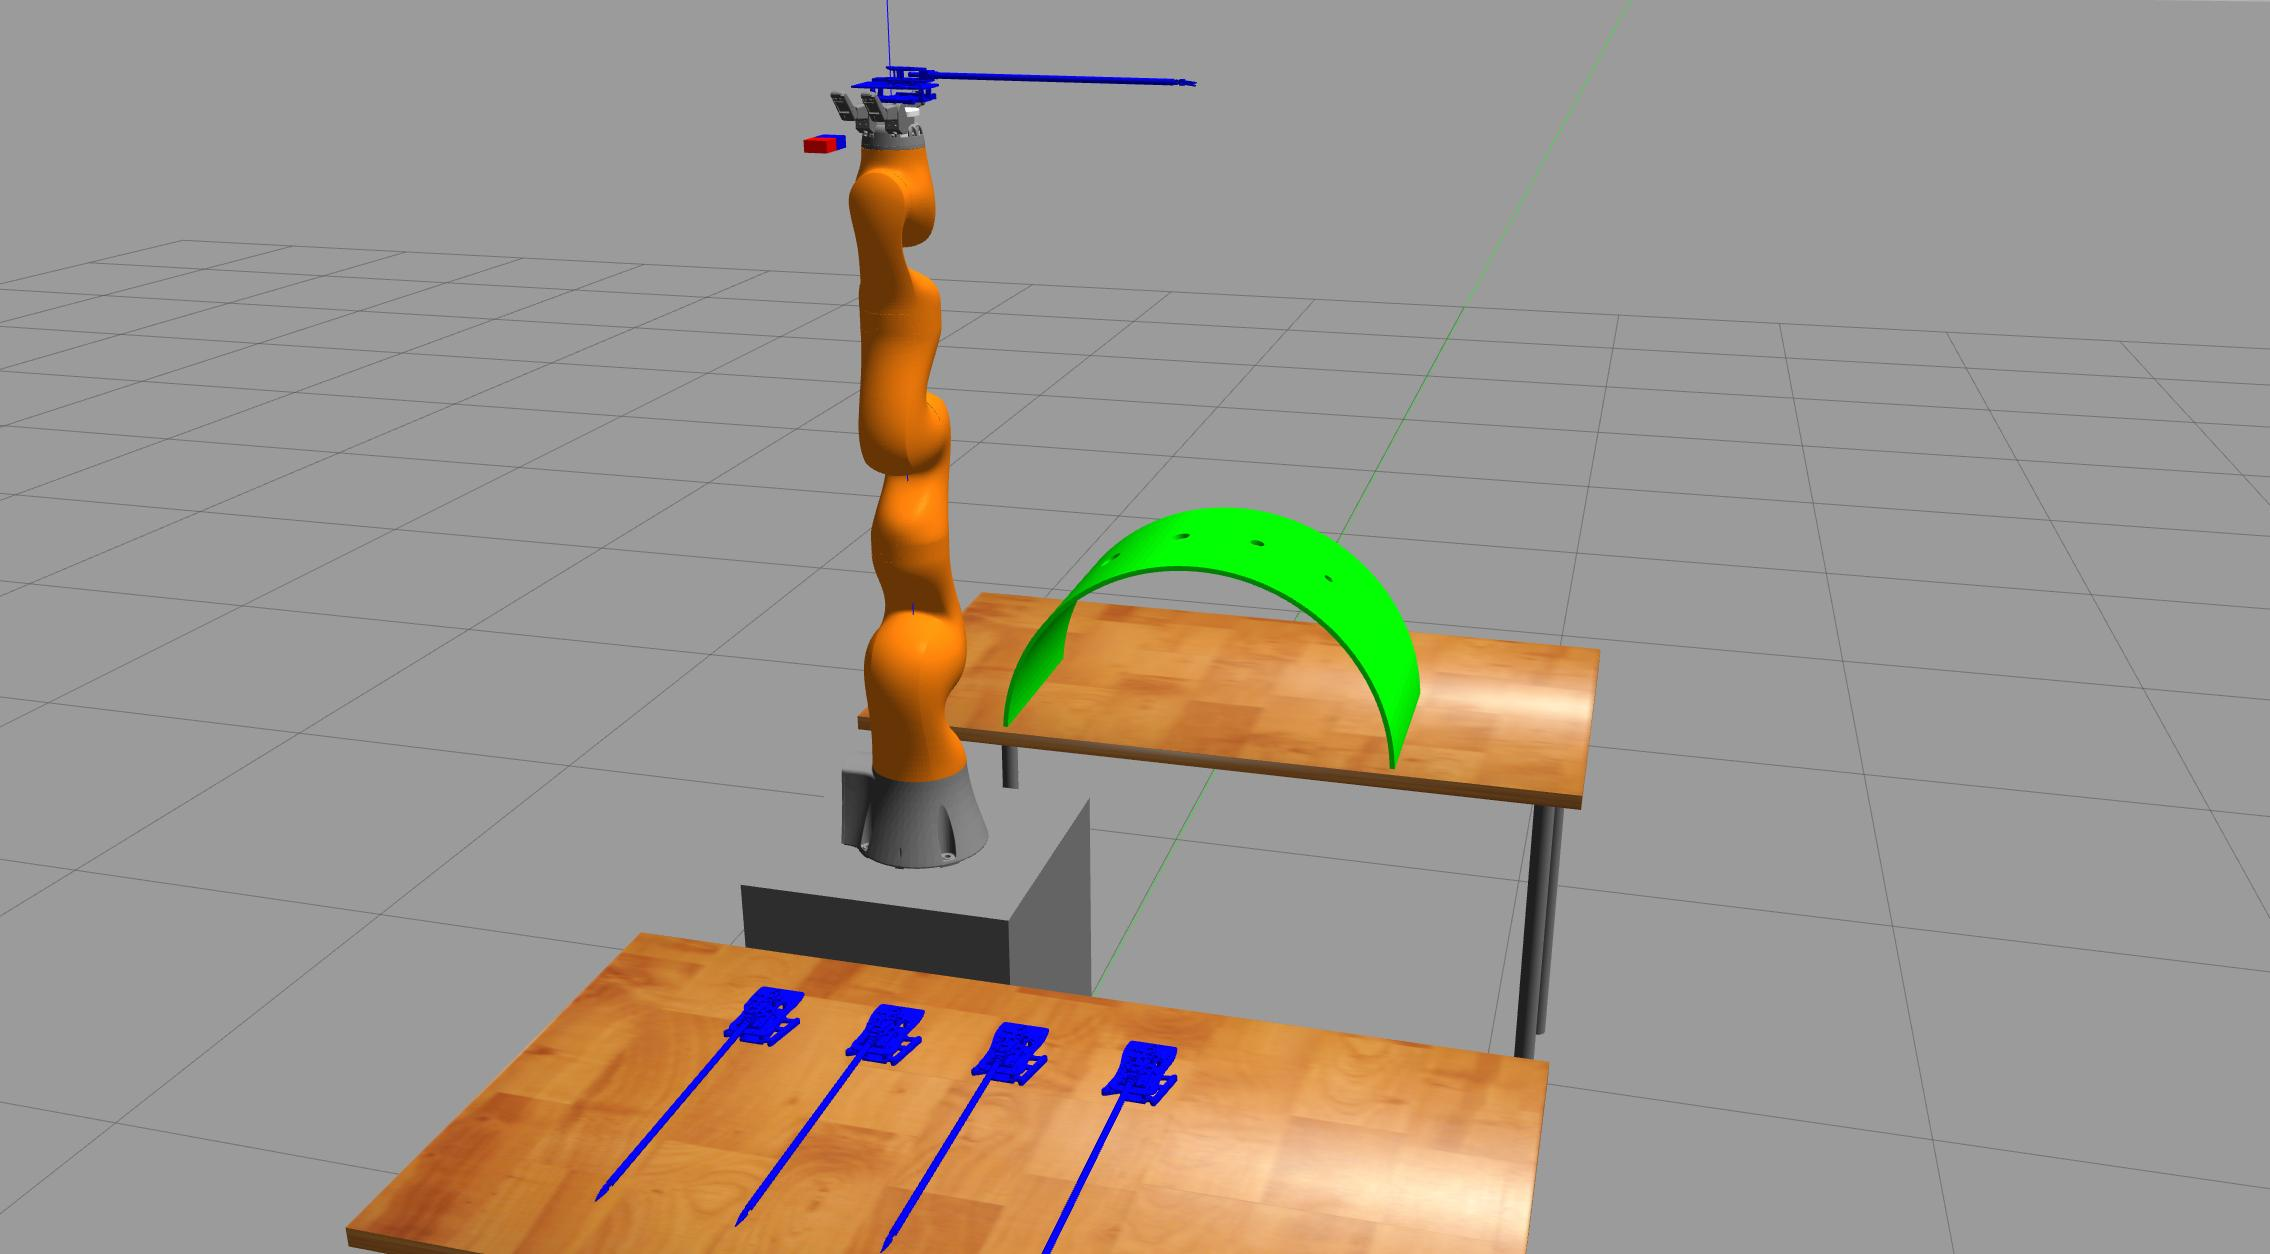
\includegraphics[width=0.3\textwidth]{images/robot_planner1/robot_planner1_1}
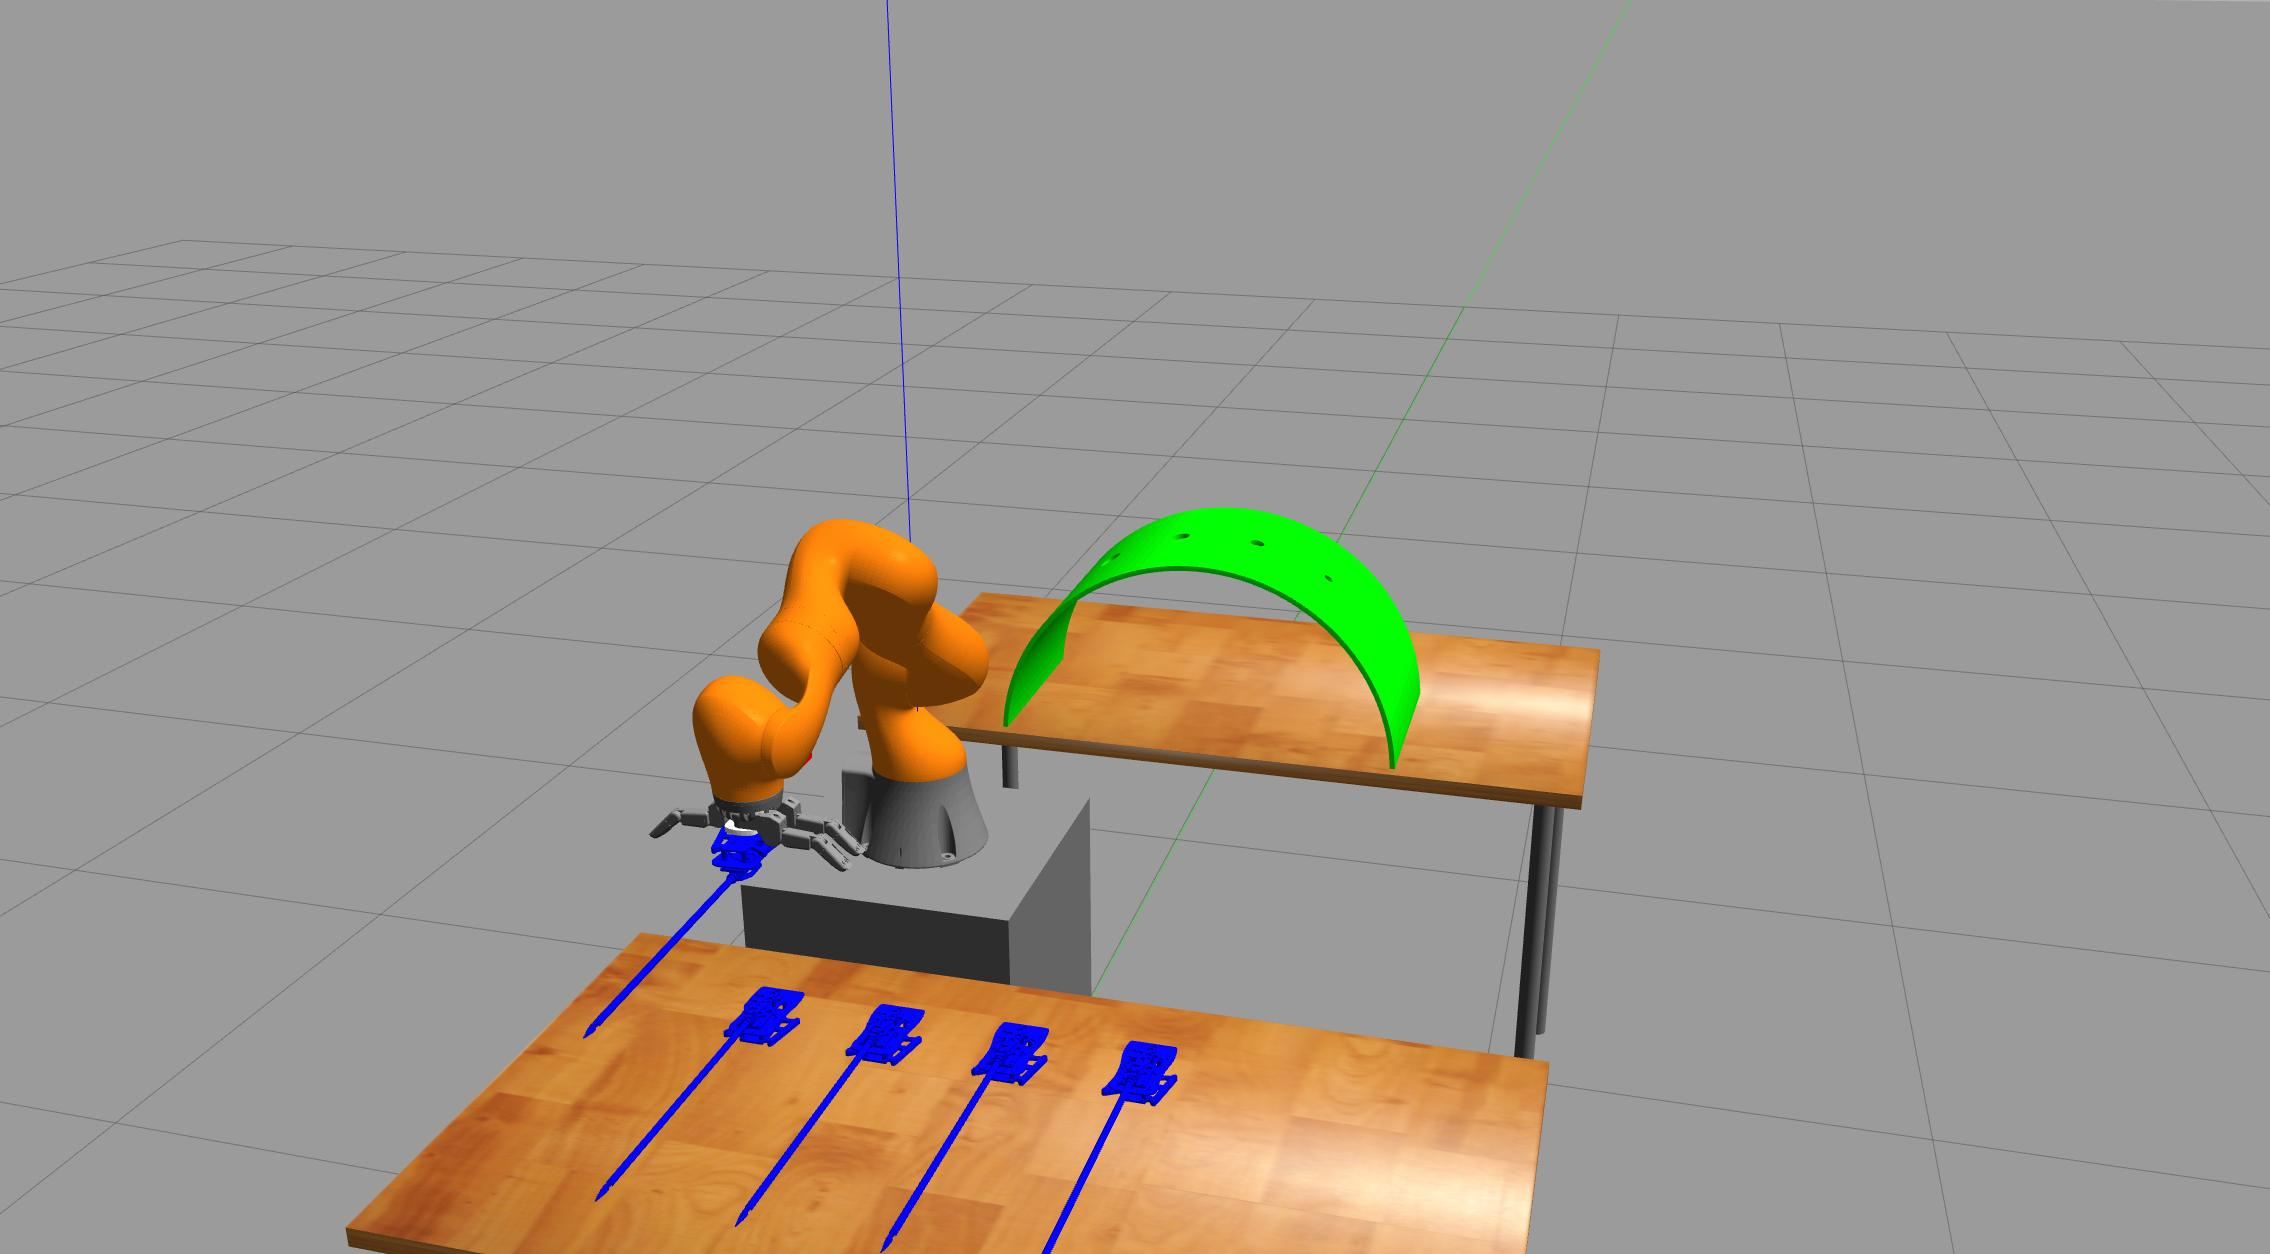
\includegraphics[width=0.3\textwidth]{images/robot_planner1/robot_planner1_2}
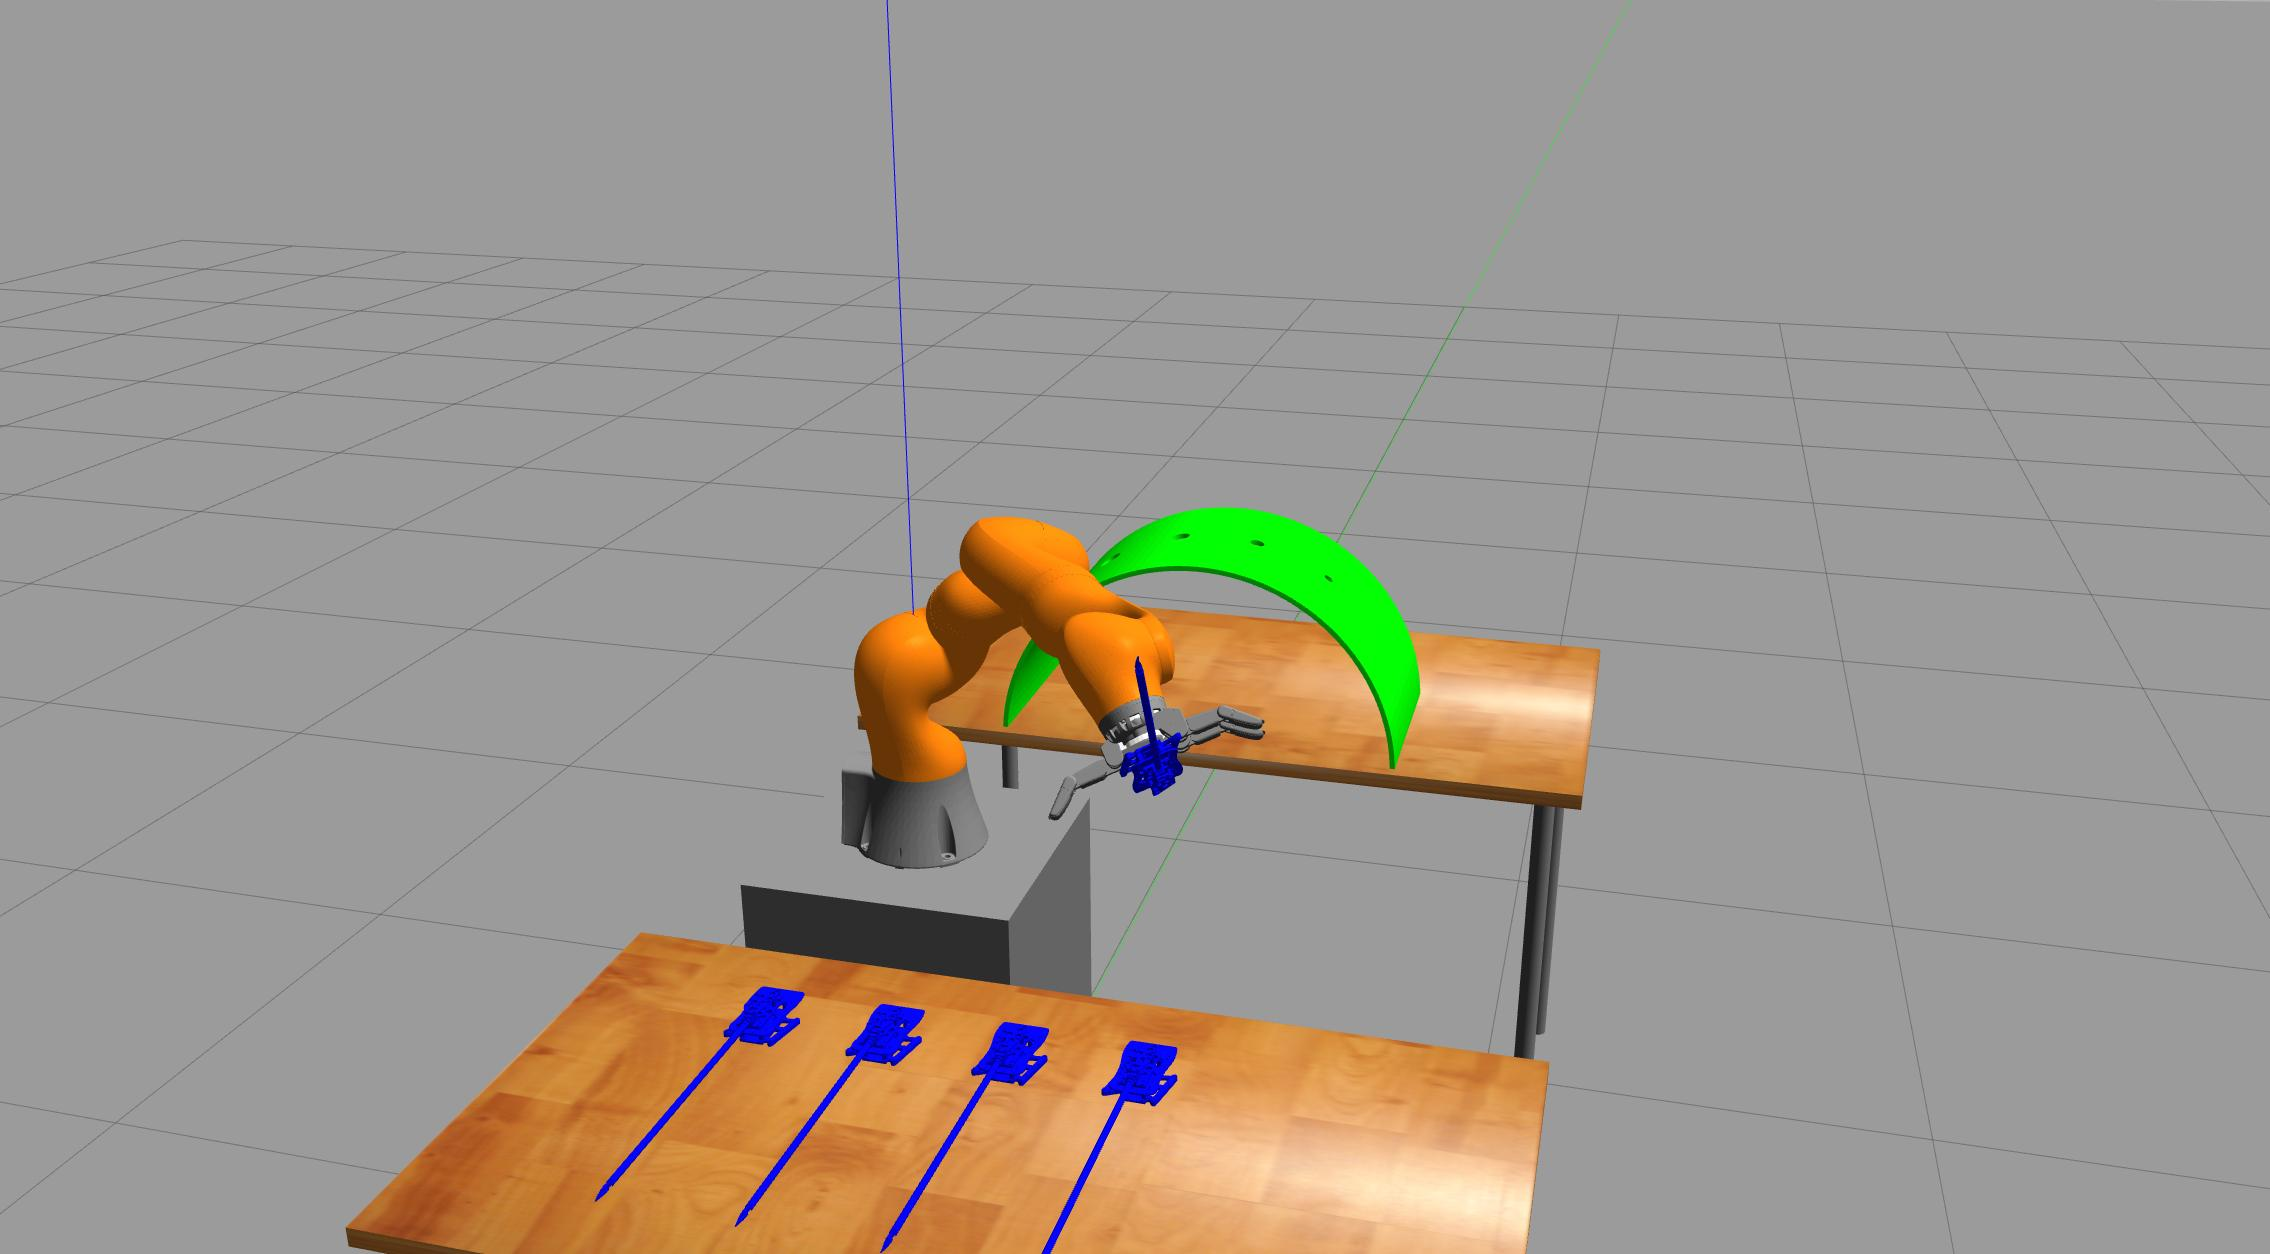
\includegraphics[width=0.3\textwidth]{images/robot_planner1/robot_planner1_3}\\
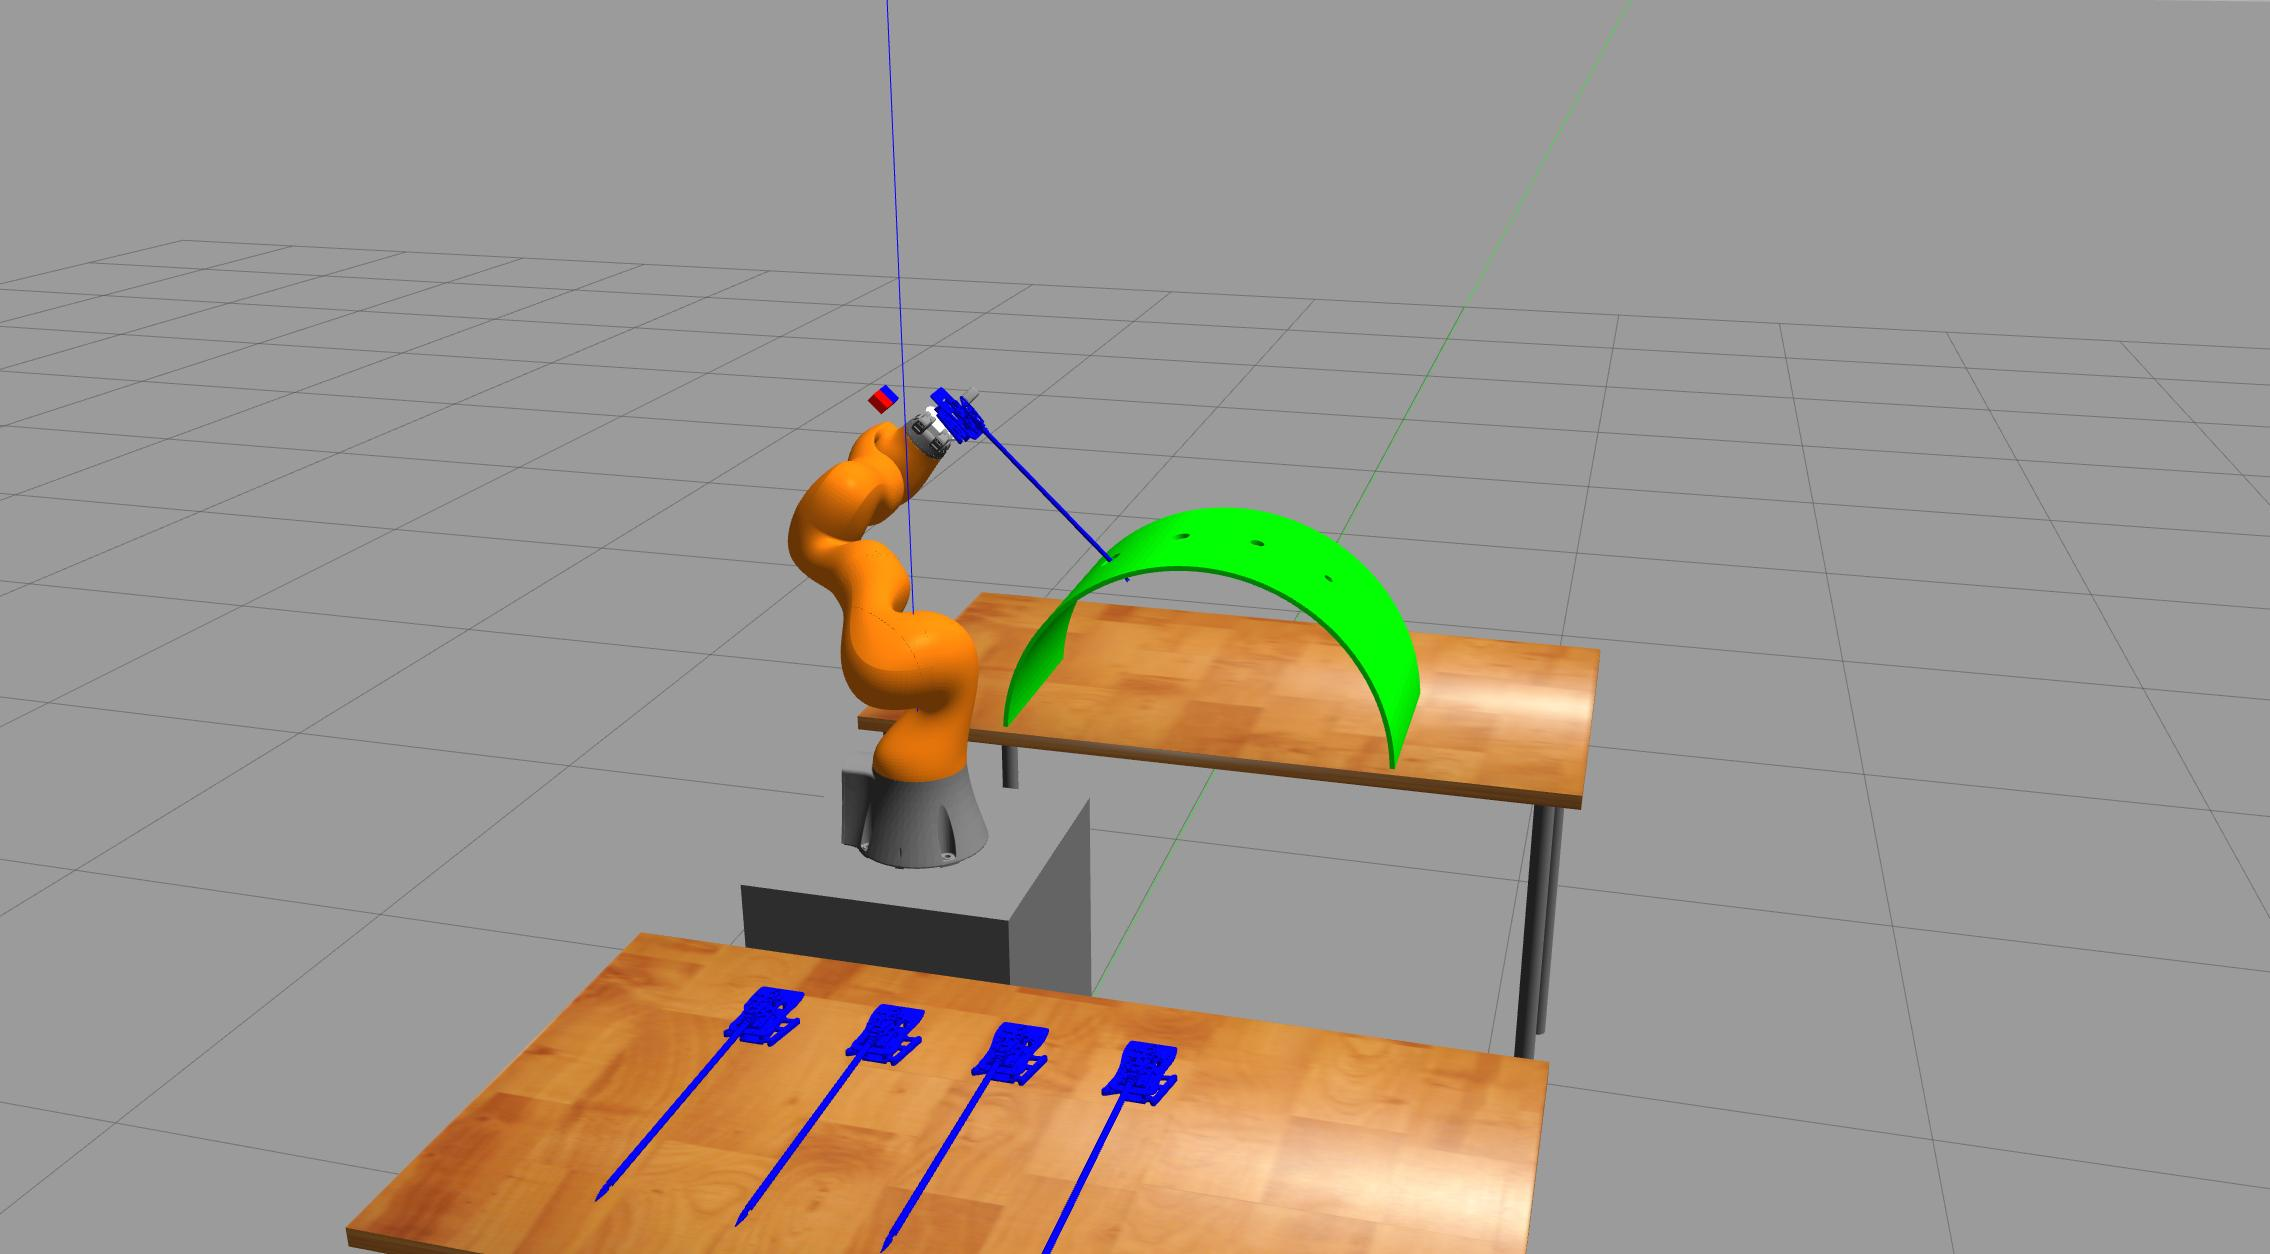
\includegraphics[width=0.3\textwidth]{images/robot_planner1/robot_planner1_4}
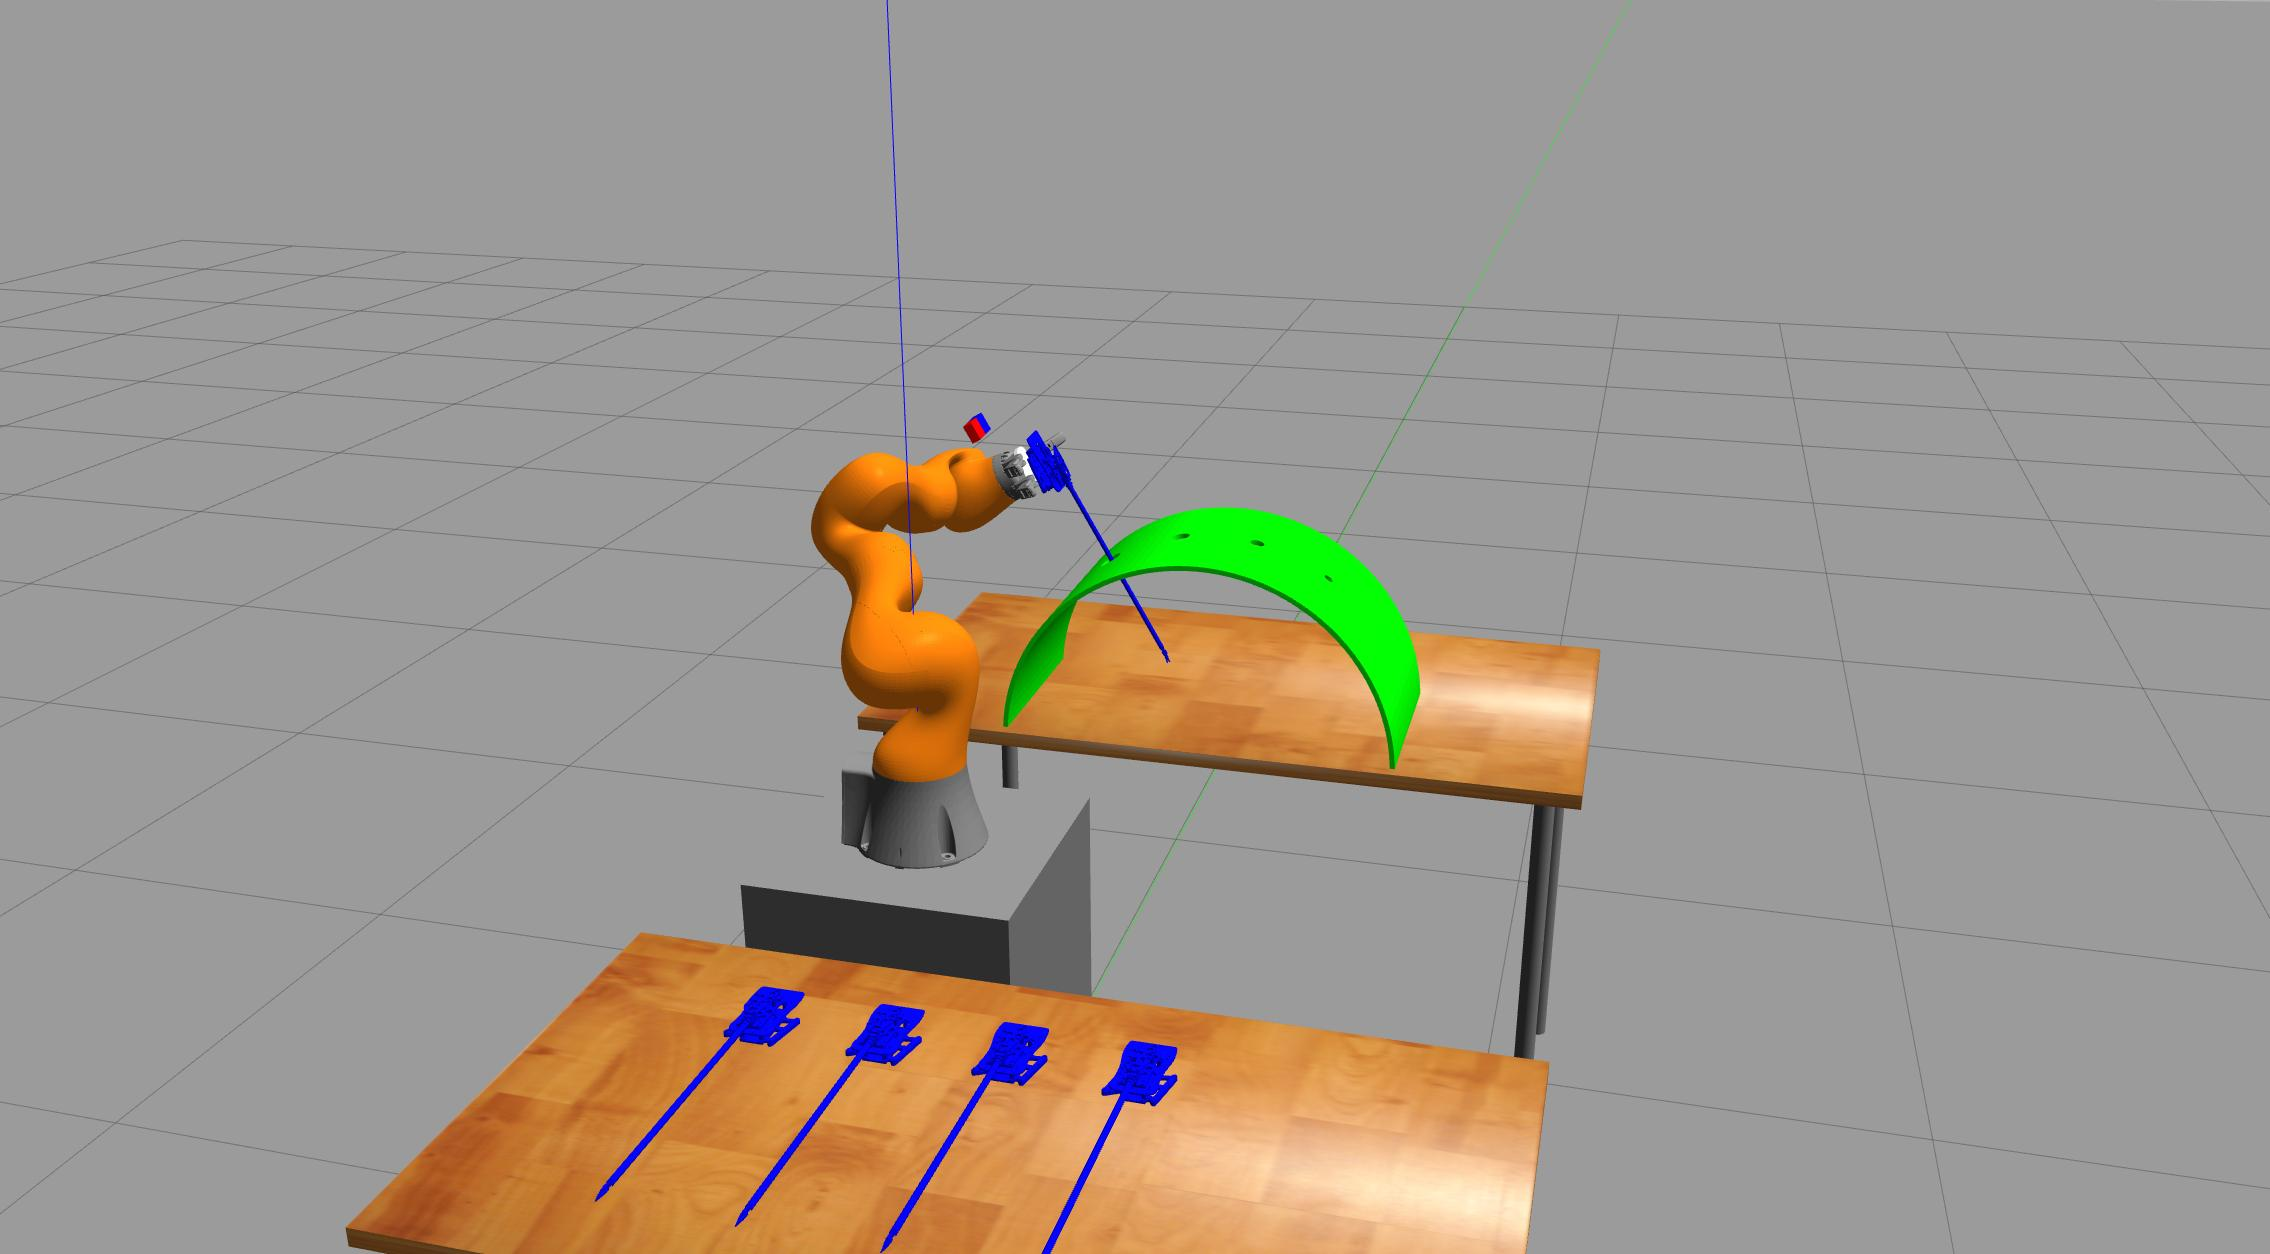
\includegraphics[width=0.3\textwidth]{images/robot_planner1/robot_planner1_5}
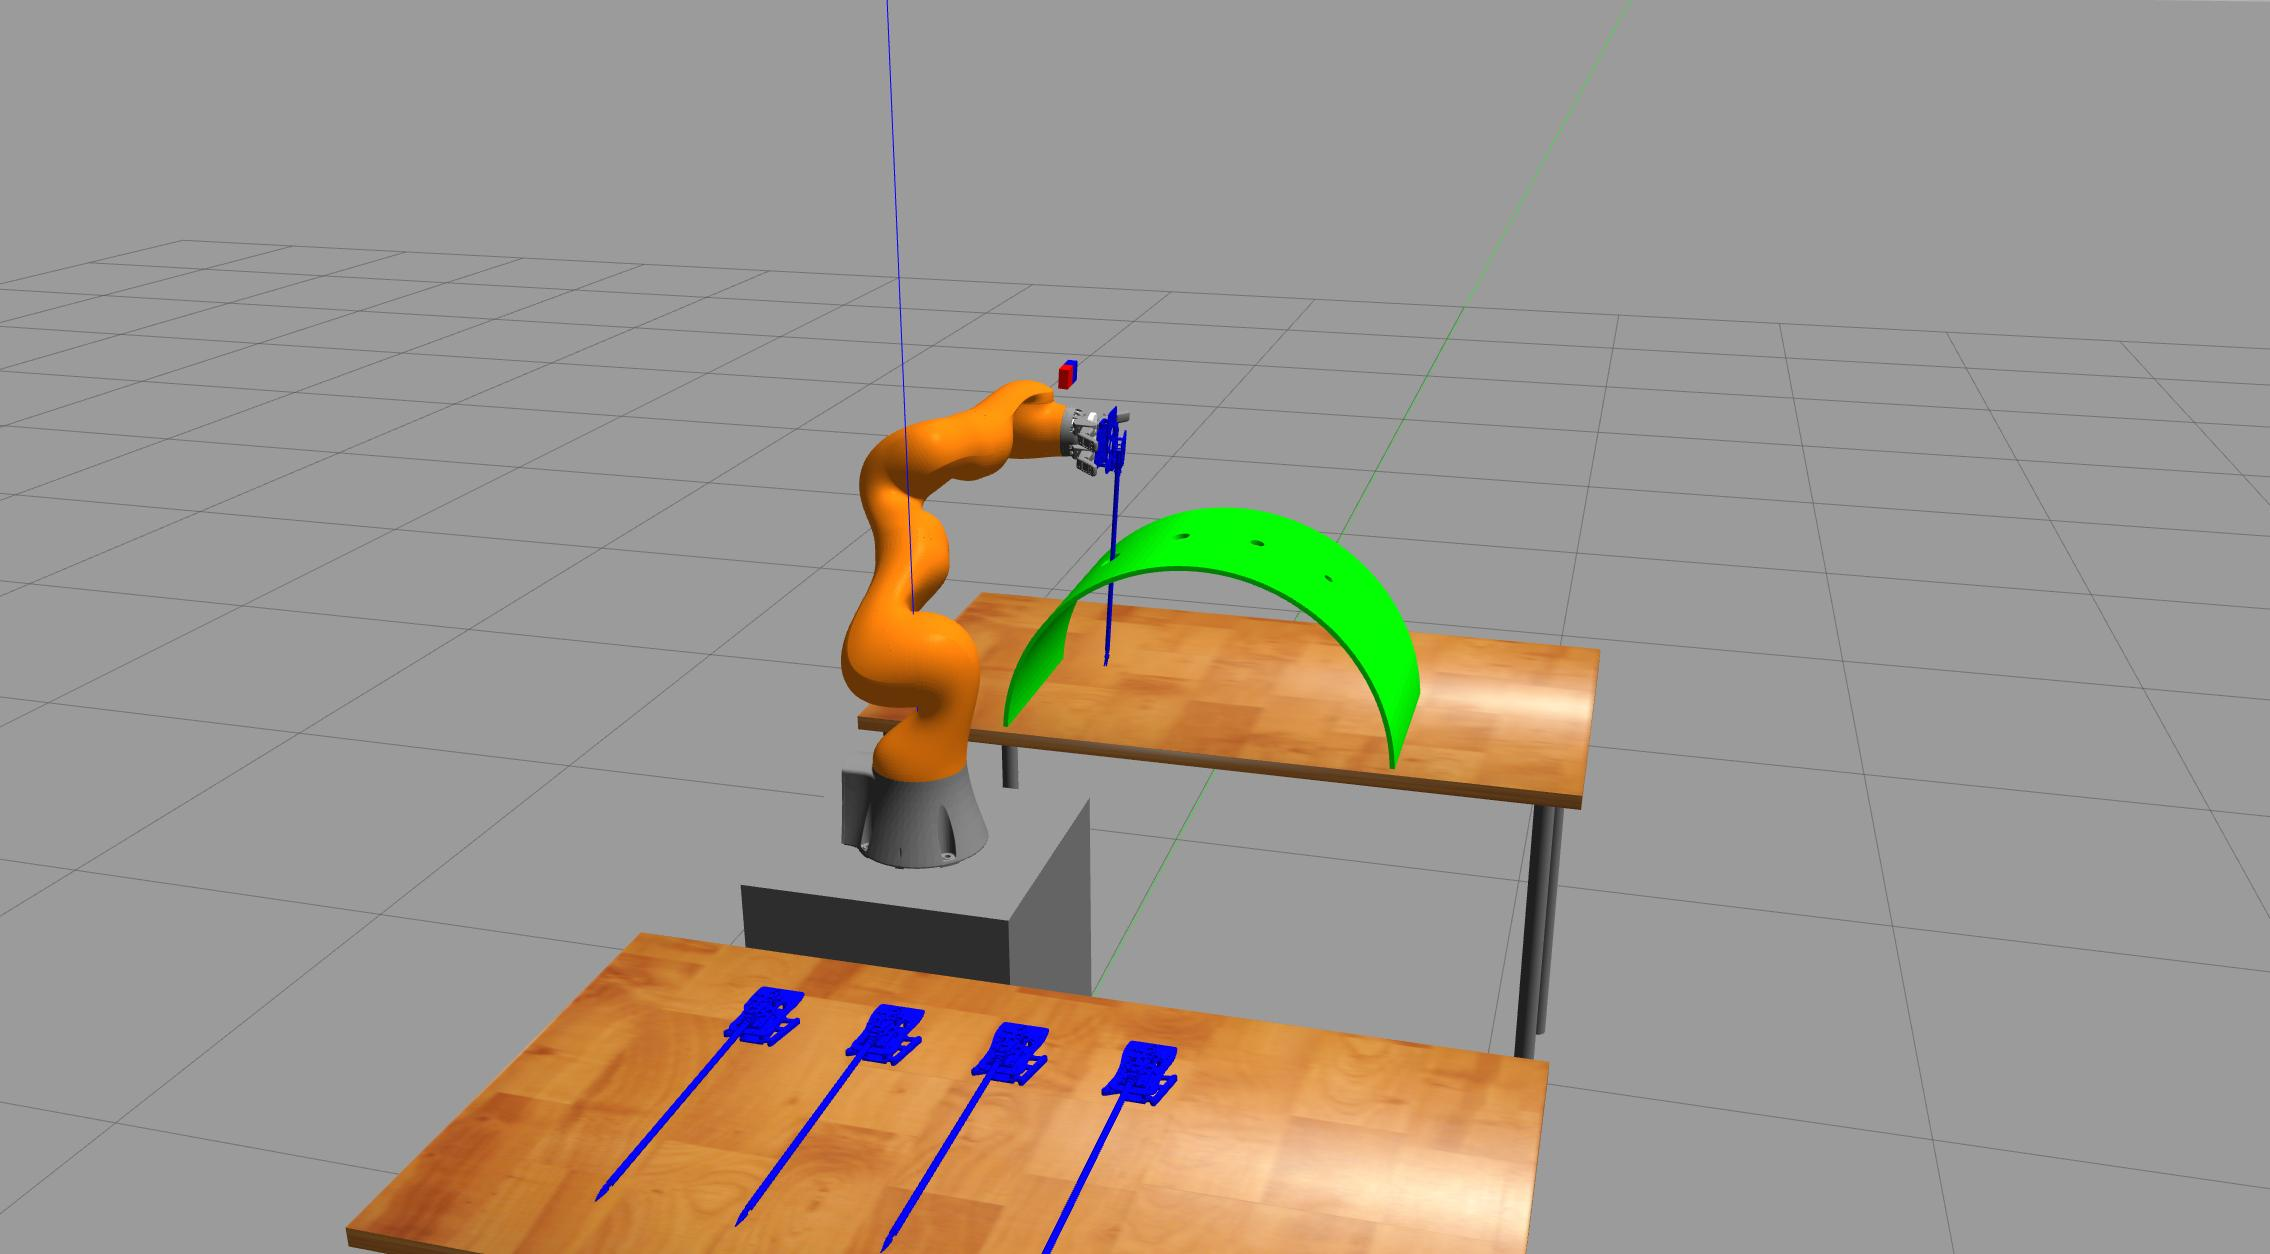
\includegraphics[width=0.3\textwidth]{images/robot_planner1/robot_planner1_6}\\
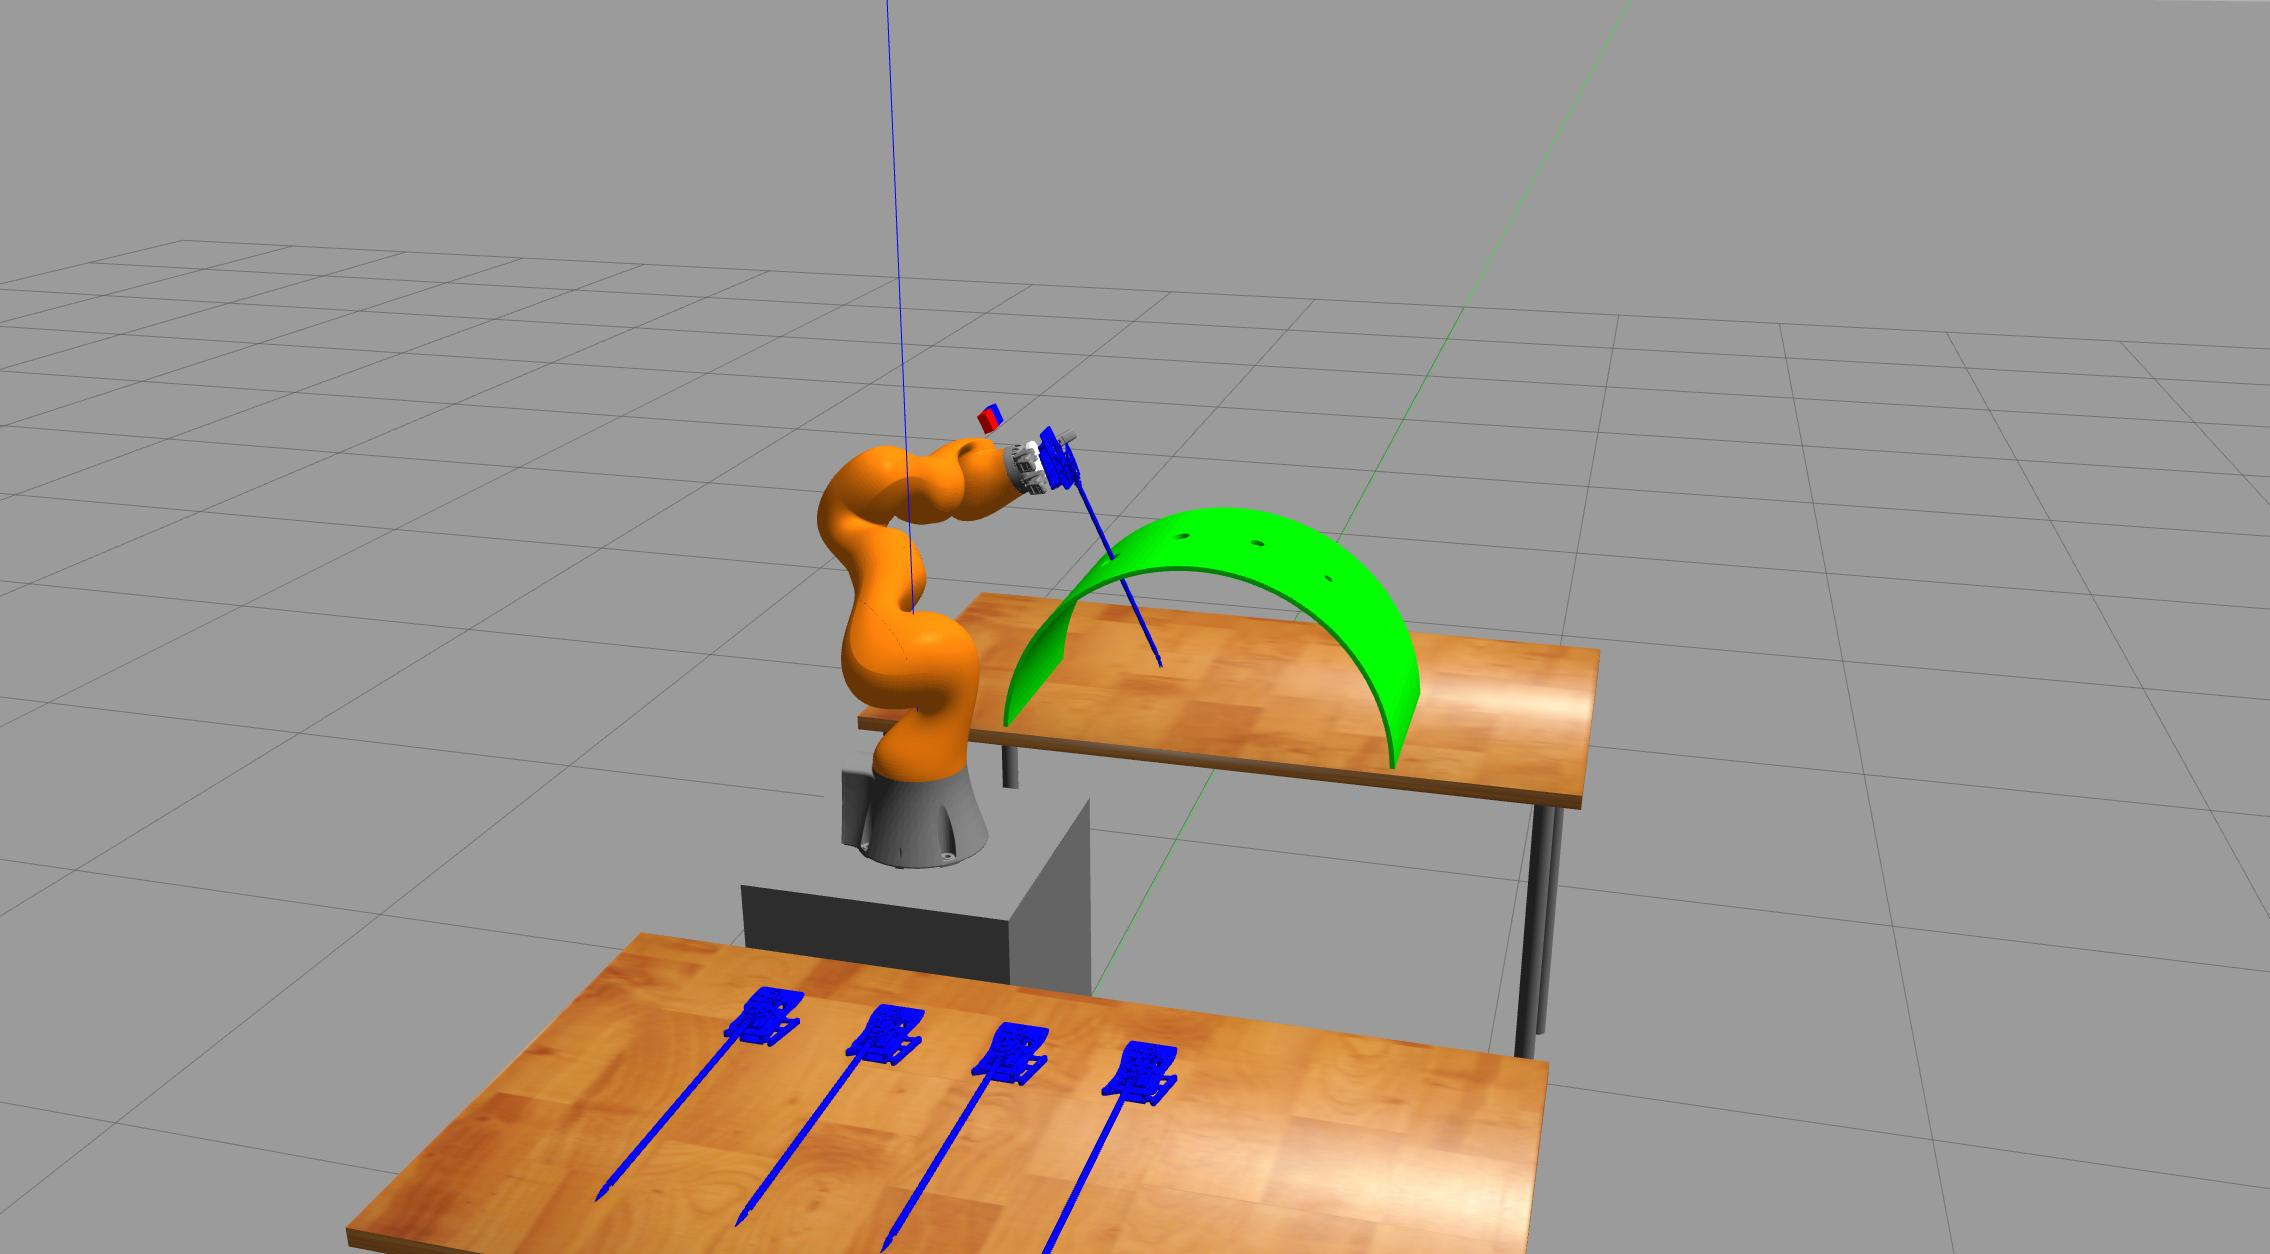
\includegraphics[width=0.3\textwidth]{images/robot_planner1/robot_planner1_7}
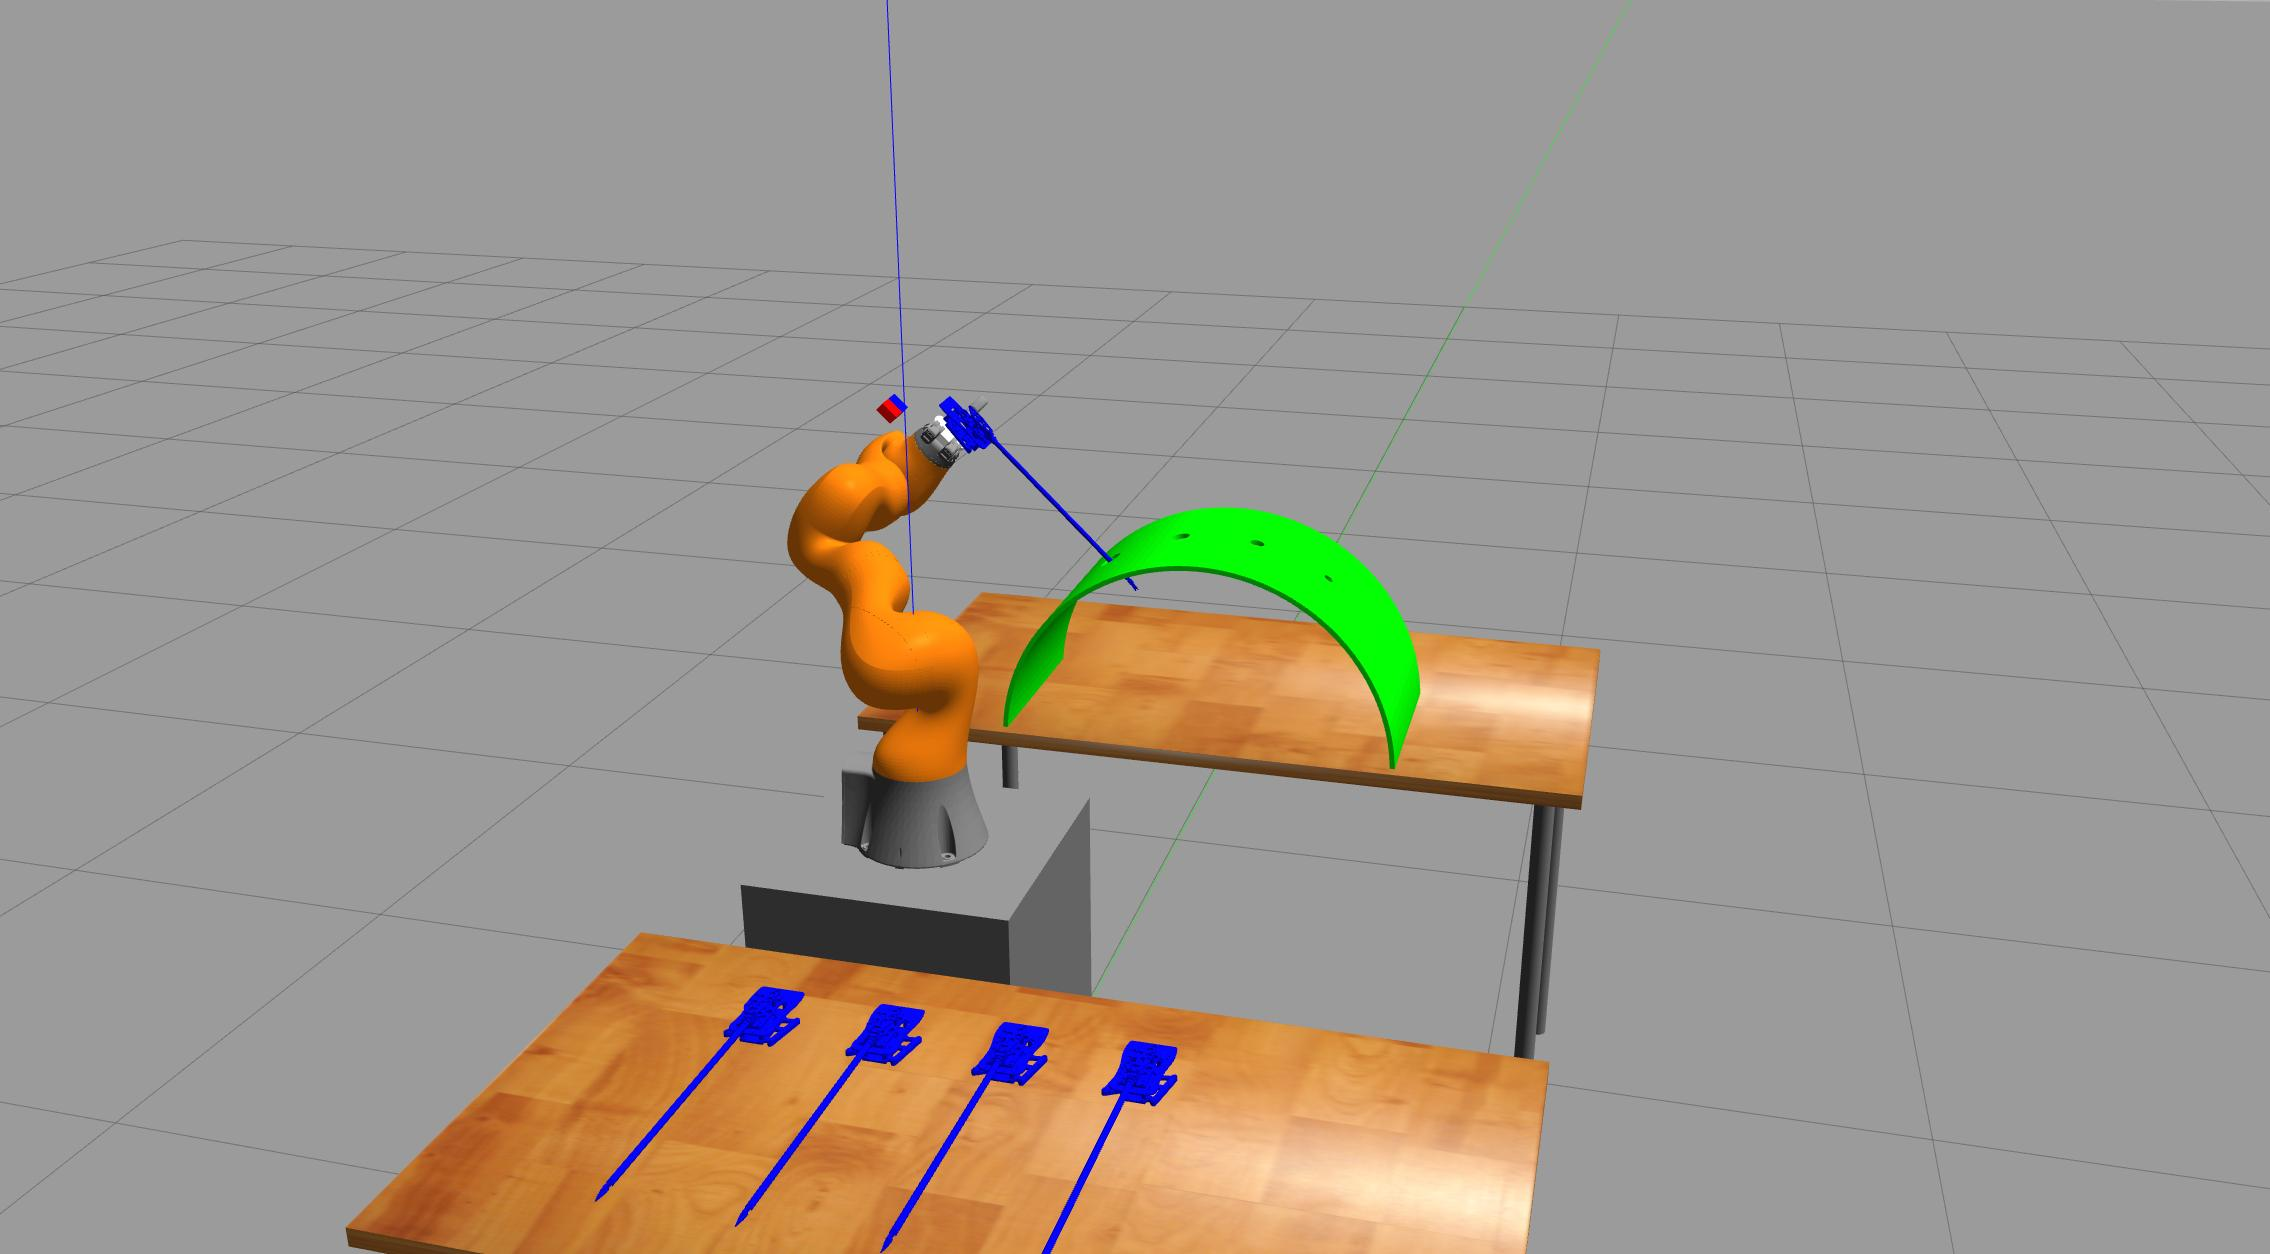
\includegraphics[width=0.3\textwidth]{images/robot_planner1/robot_planner1_8}
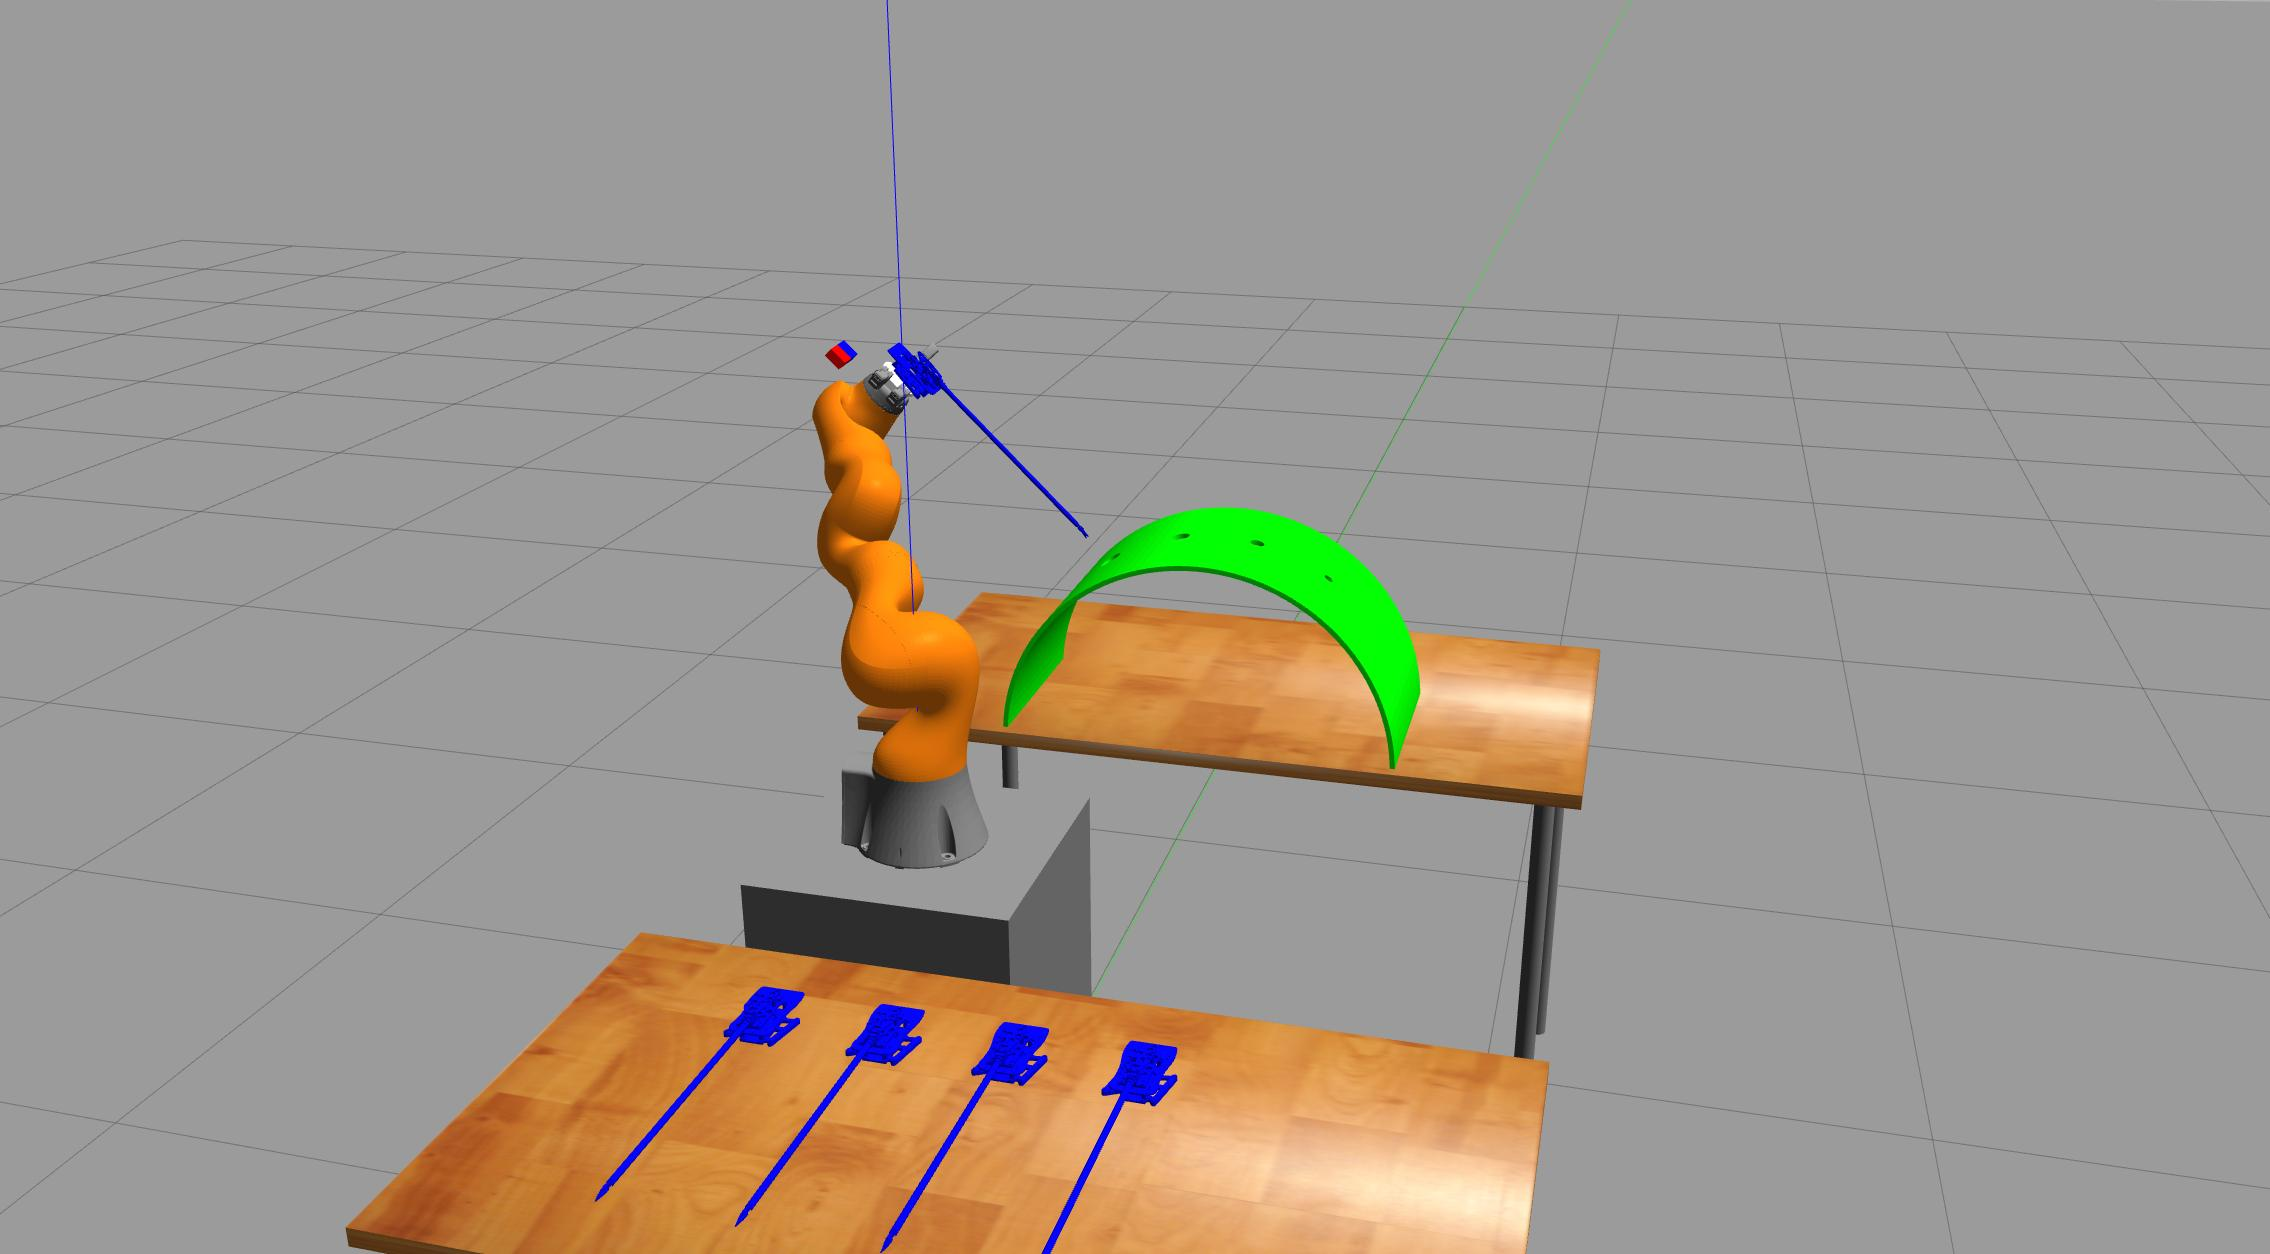
\includegraphics[width=0.3\textwidth]{images/robot_planner1/robot_planner1_9}\\
\caption{Experiment 1:}
\end{figure}
\end{center}


\subsubsection{Robot Planner 2}

In this experiment, we plan a path such that the robot arm will visit all holes of the mounting dock and will try the insertion movement of the surgical tool.
This experiment is very useful, because it shows whether all holes of the mounting dock are \textbf{reachable} (inside the robot's work space) and if so, how 
\textbf{dexterous} the robot will be in pivoting around each hole, i.e. how free the robot arm is to execute pivot motions.

\begin{center}
\begin{figure}[H]
\centering
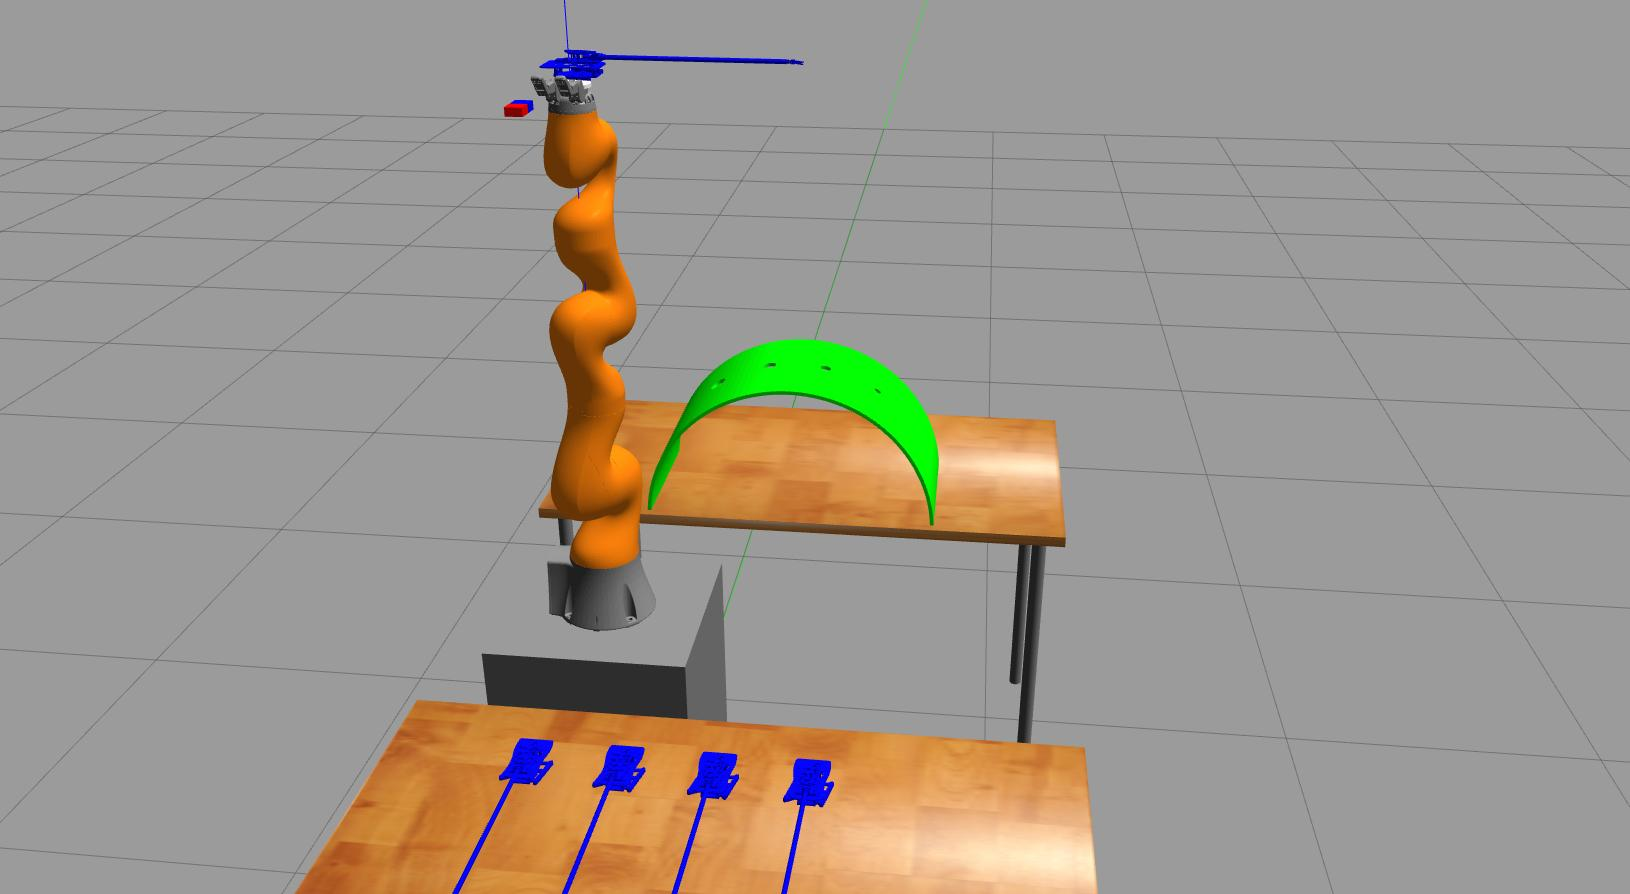
\includegraphics[width=0.3\textwidth]{images/robot_planner2/robot_planner2_1}
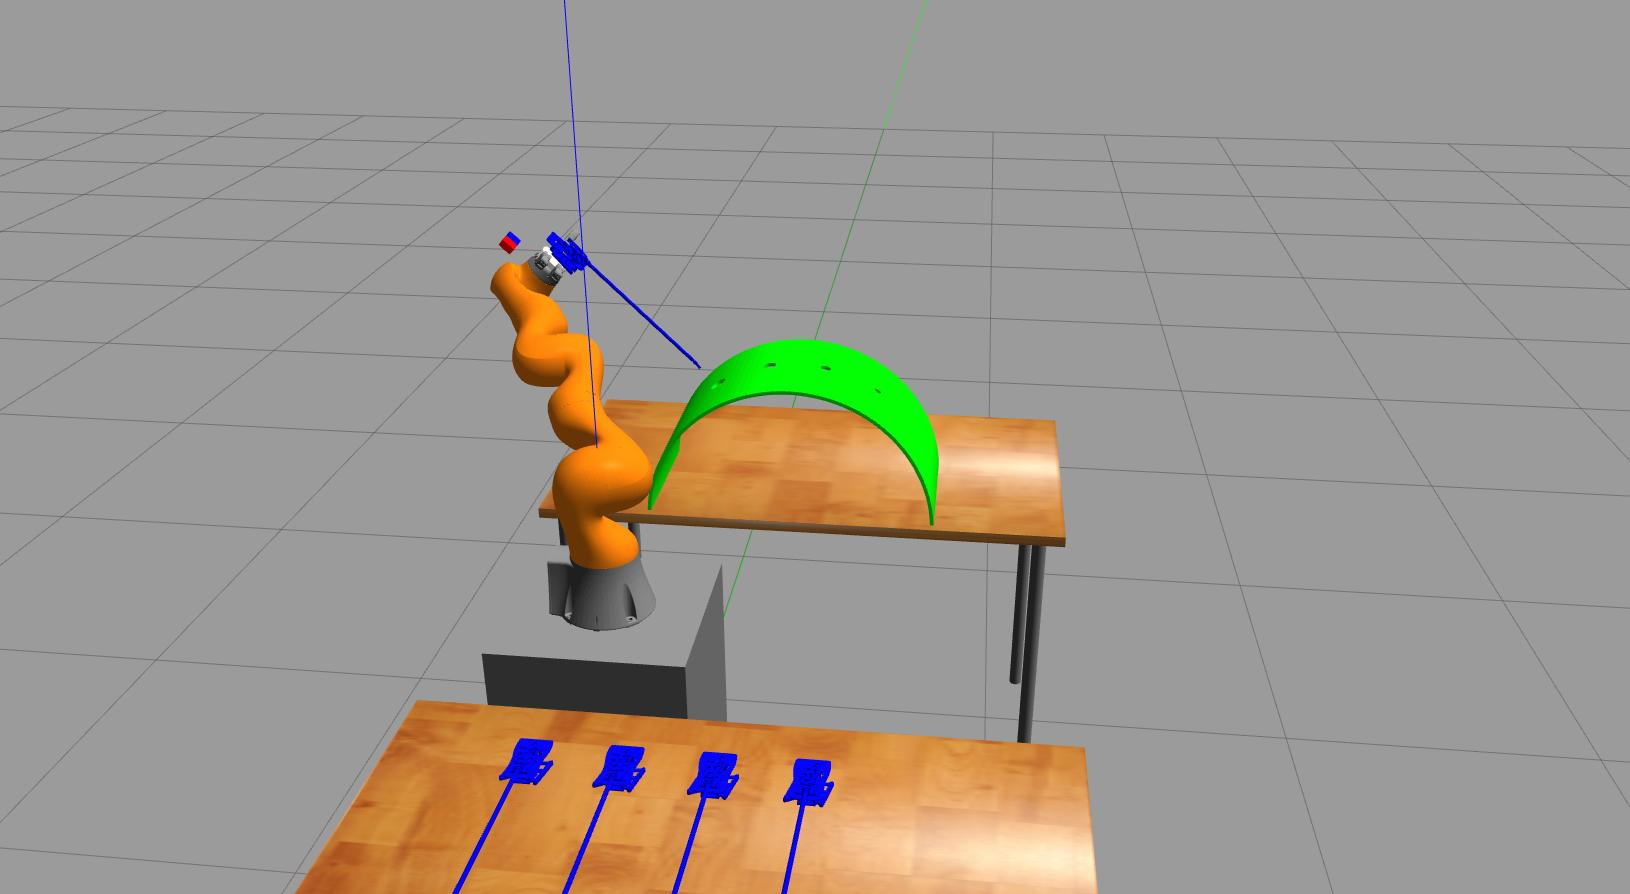
\includegraphics[width=0.3\textwidth]{images/robot_planner2/robot_planner2_2}
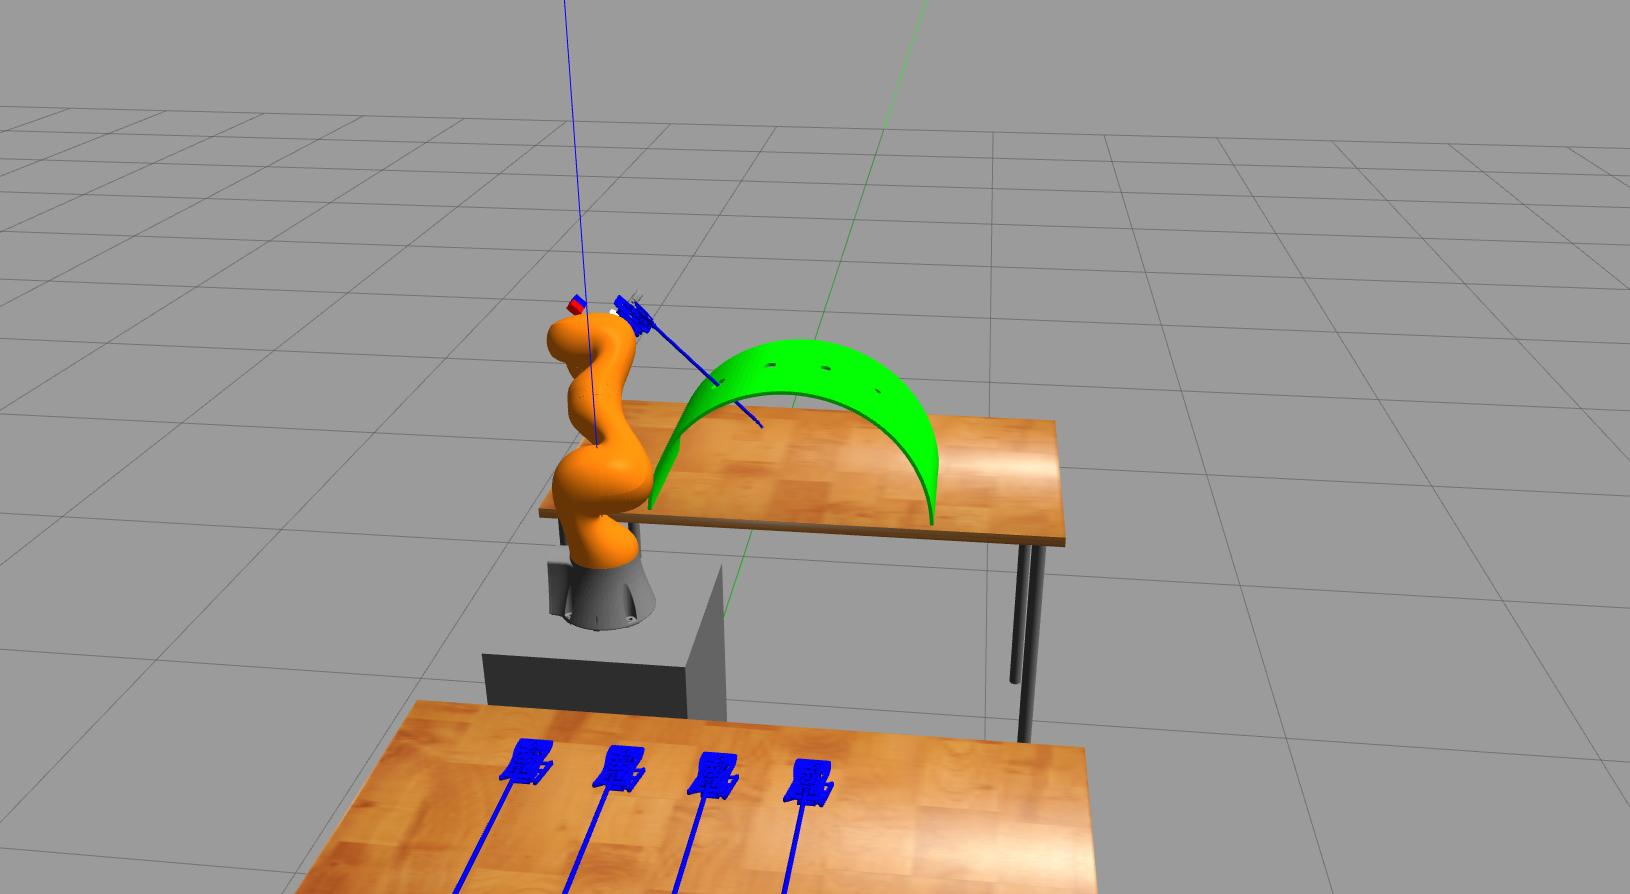
\includegraphics[width=0.3\textwidth]{images/robot_planner2/robot_planner2_3}\\
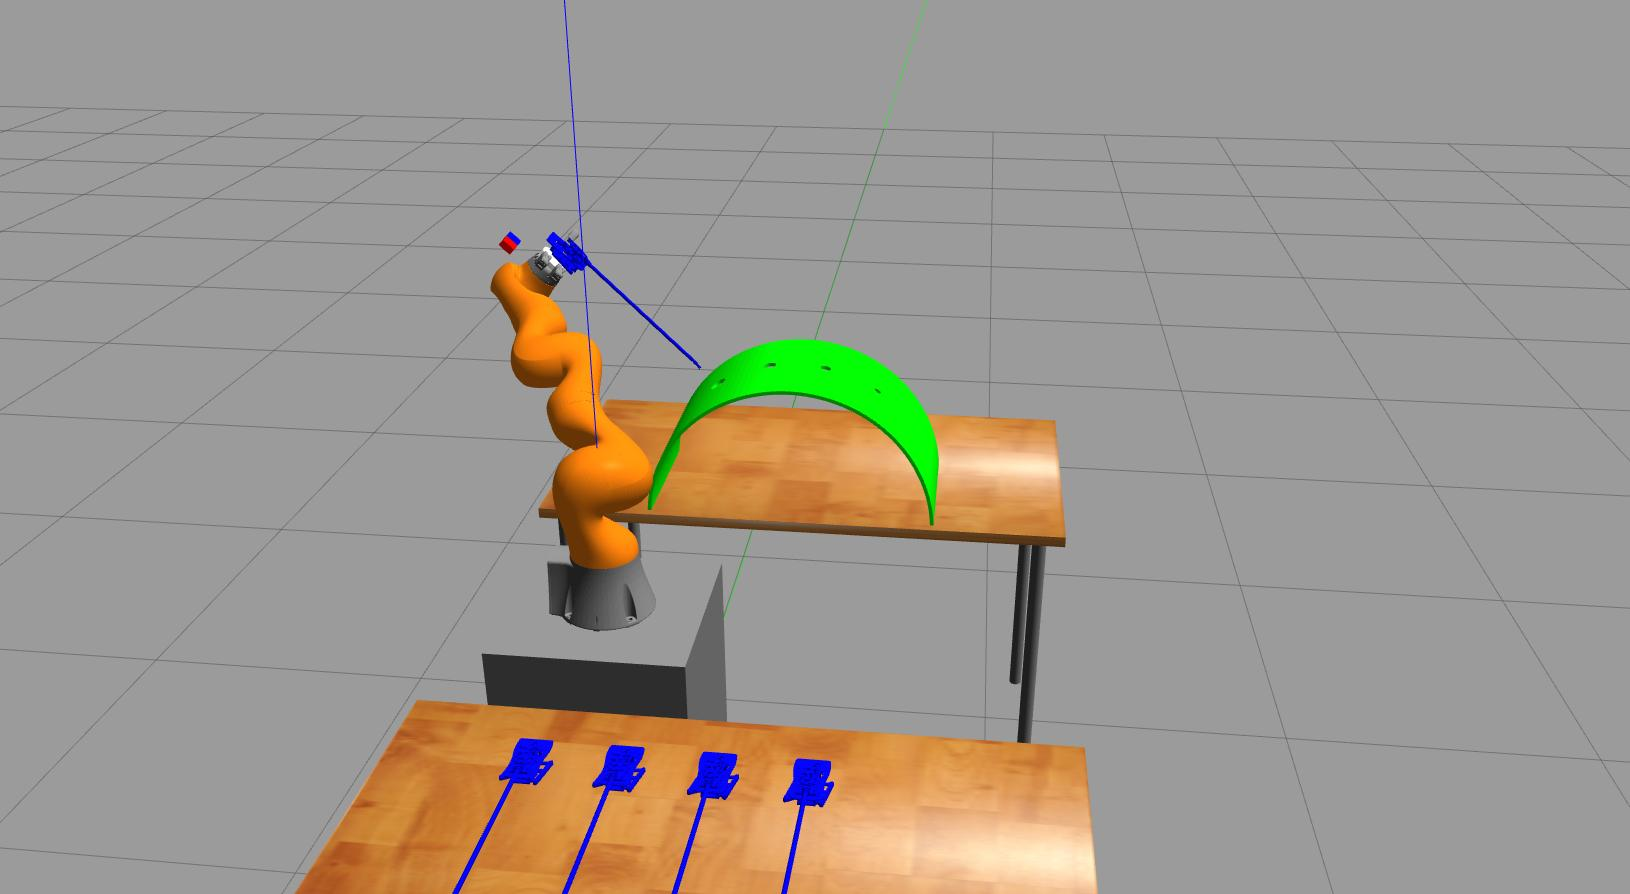
\includegraphics[width=0.3\textwidth]{images/robot_planner2/robot_planner2_4}
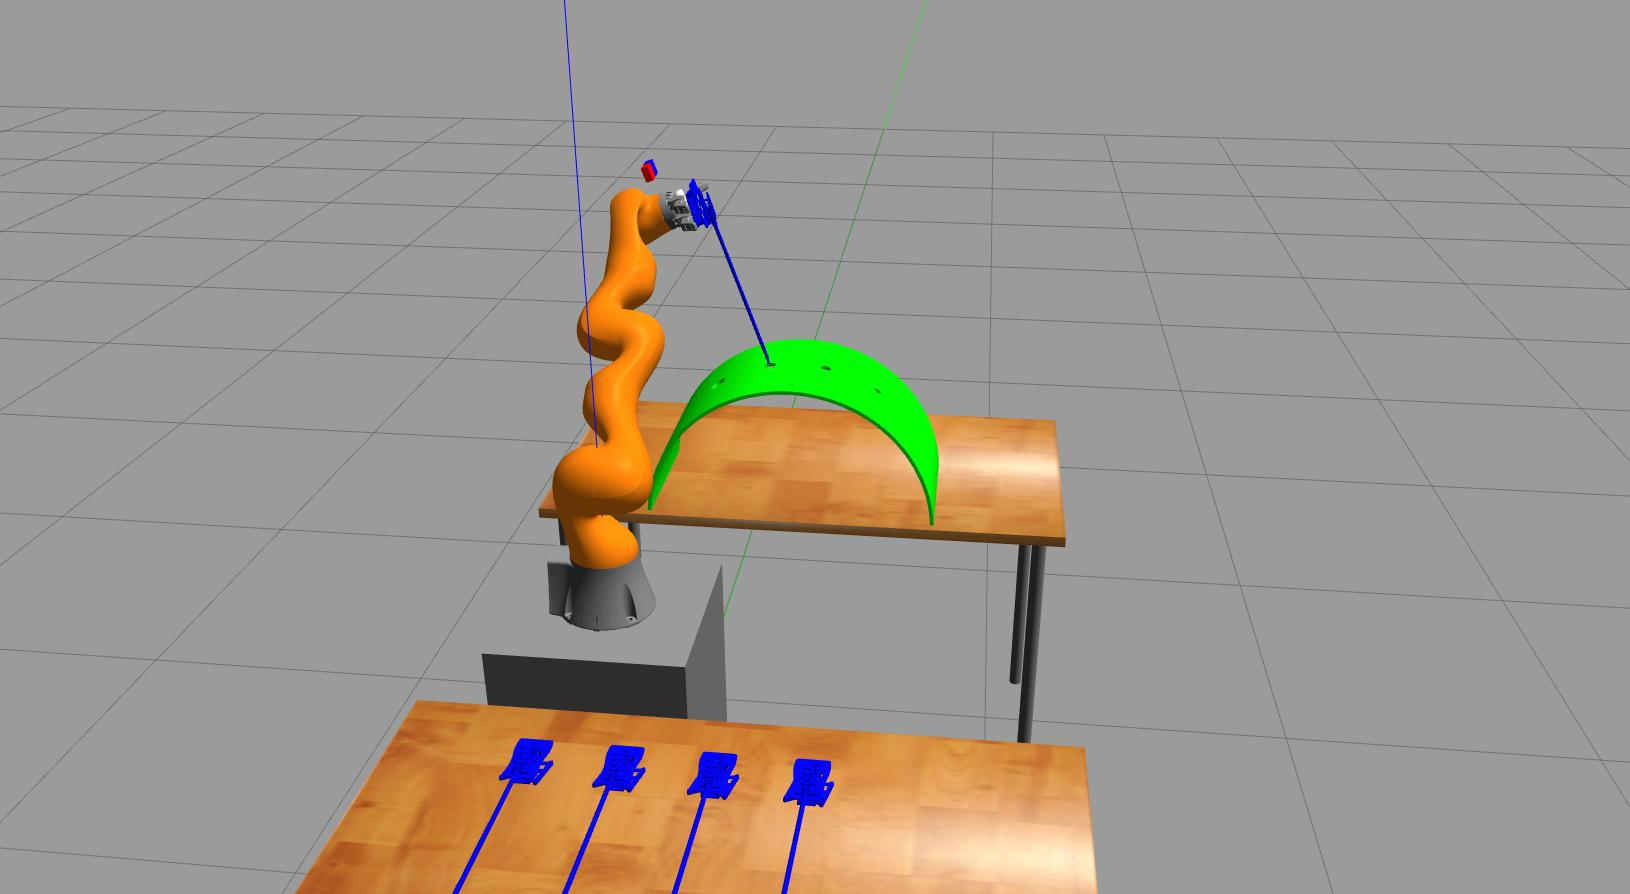
\includegraphics[width=0.3\textwidth]{images/robot_planner2/robot_planner2_5}
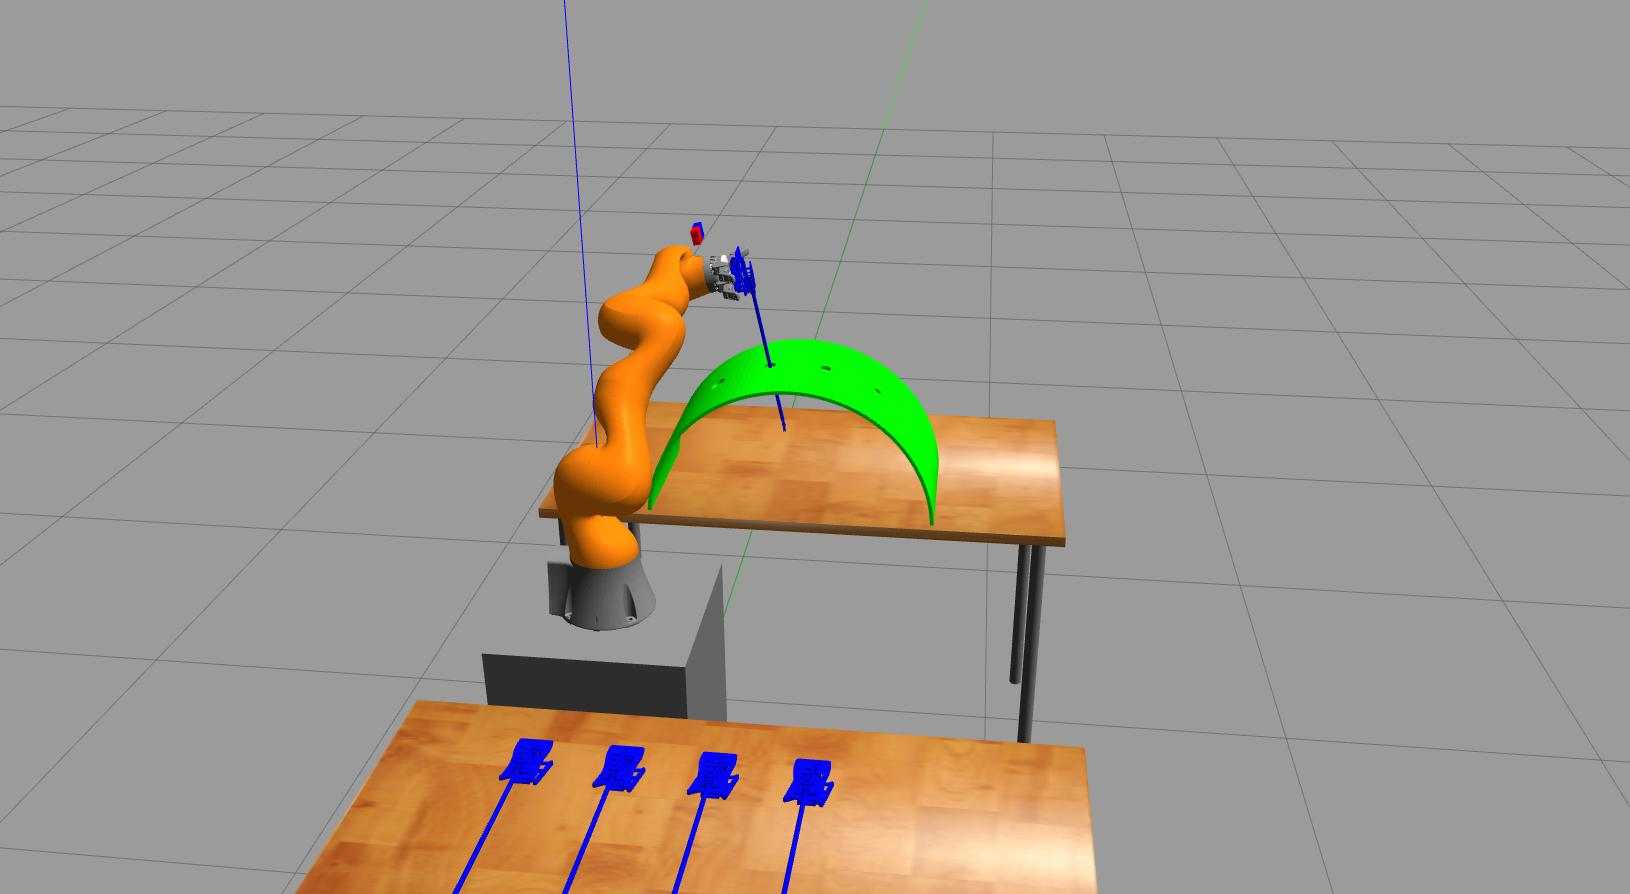
\includegraphics[width=0.3\textwidth]{images/robot_planner2/robot_planner2_6}\\
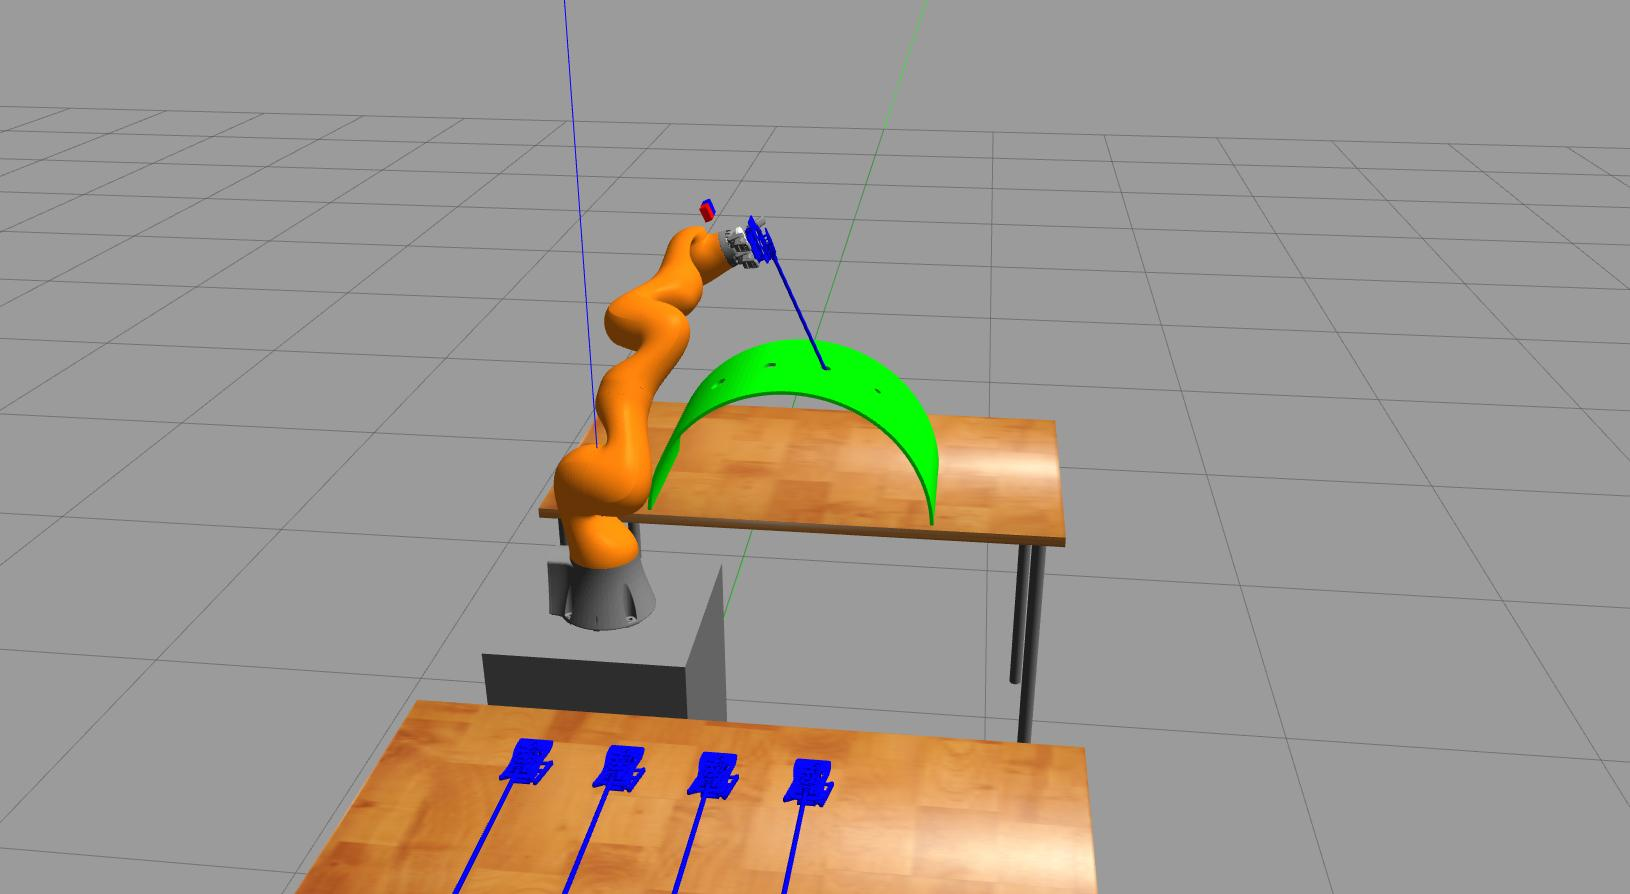
\includegraphics[width=0.3\textwidth]{images/robot_planner2/robot_planner2_7}
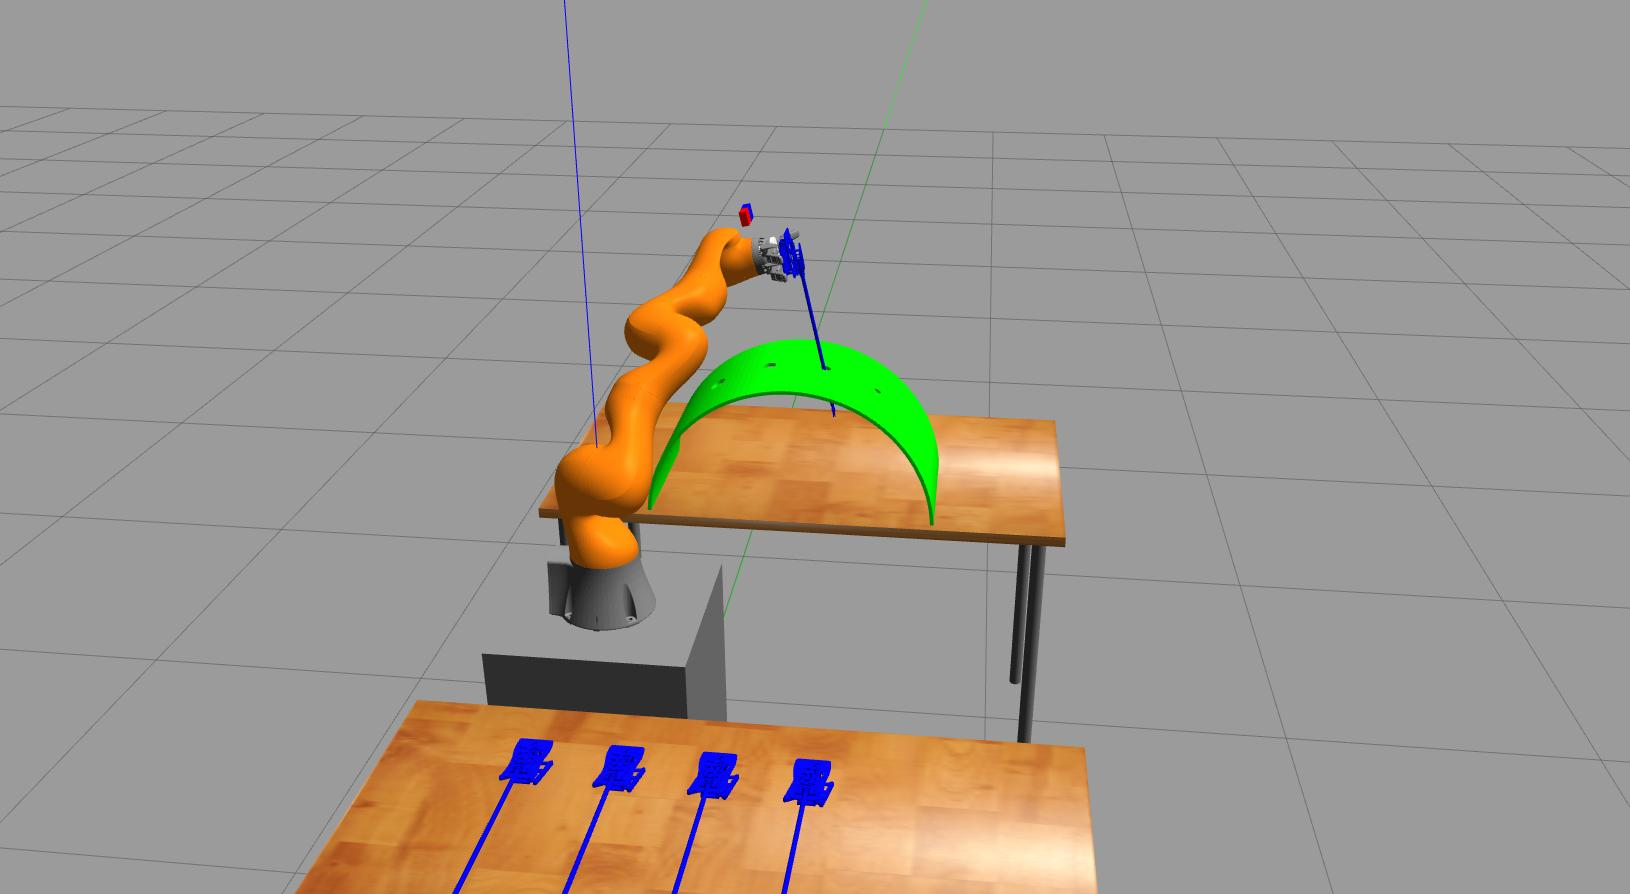
\includegraphics[width=0.3\textwidth]{images/robot_planner2/robot_planner2_8}\\
\caption{Experiment 2a:}
\label{experiment-robot-planner2a}
\end{figure}
\end{center}

To overcome the reachability issue shown in Figure \ref{experiment-robot-planner2a}, the algorithm was repeated, but this time using a different simulation layout 
in Gazebo, in which the mounting dock is closer to the robot and in front of it. This new layout enables the robot to reach all mounting holes with ease and 
with sufficient dexterity, the robot is free to pivot around.

\begin{center}
\begin{figure}[H]
\centering
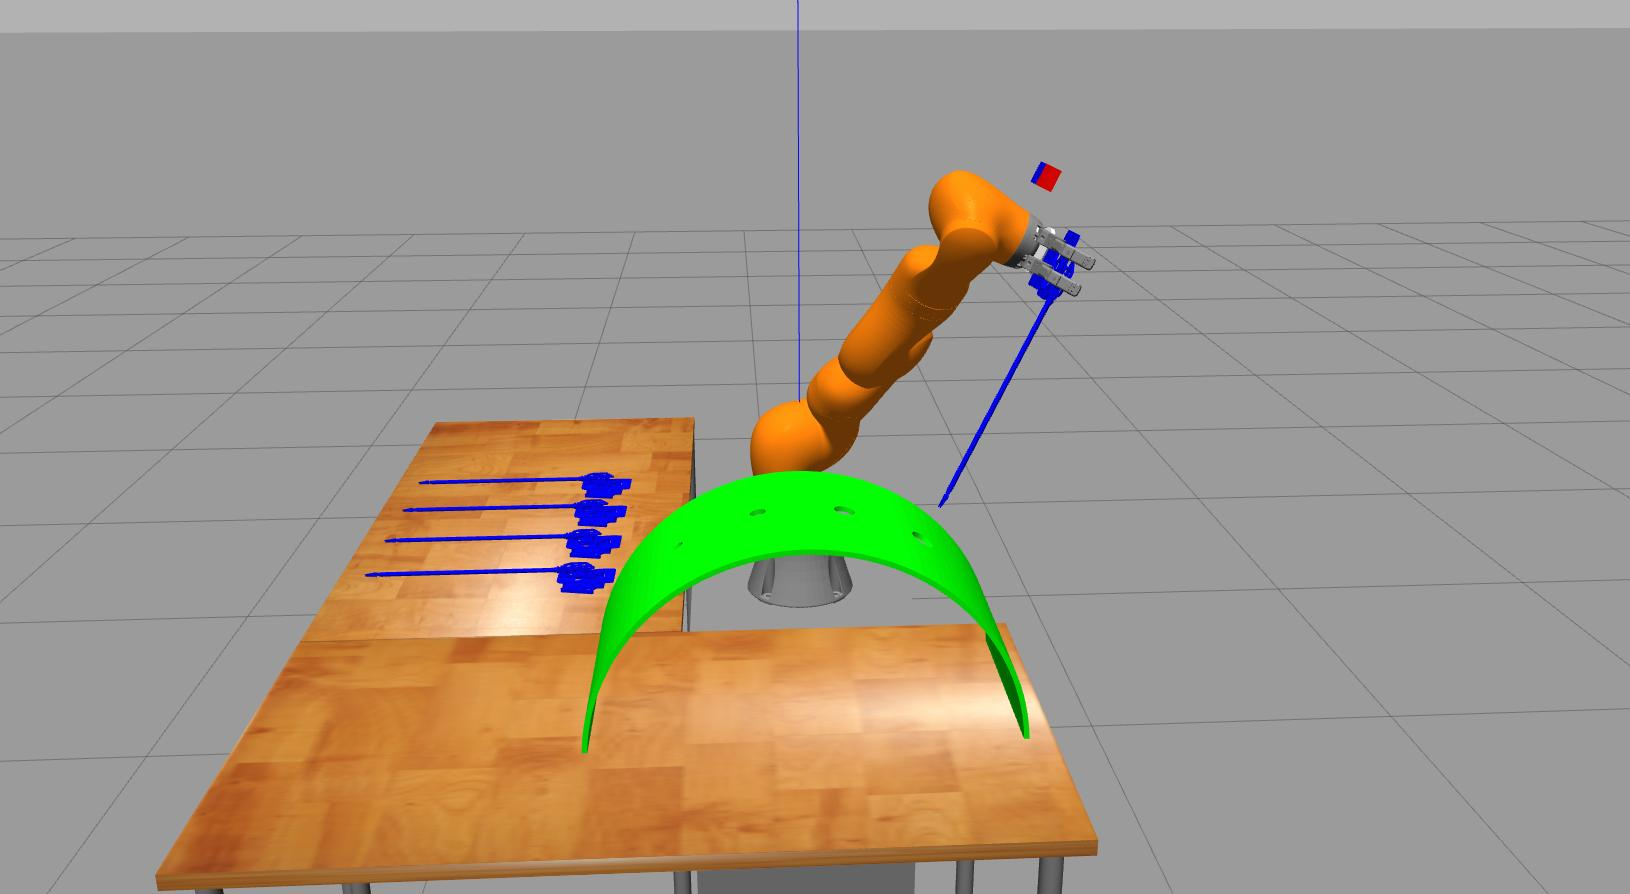
\includegraphics[width=0.3\textwidth]{images/robot_planner2b/robot_planner2b_1}
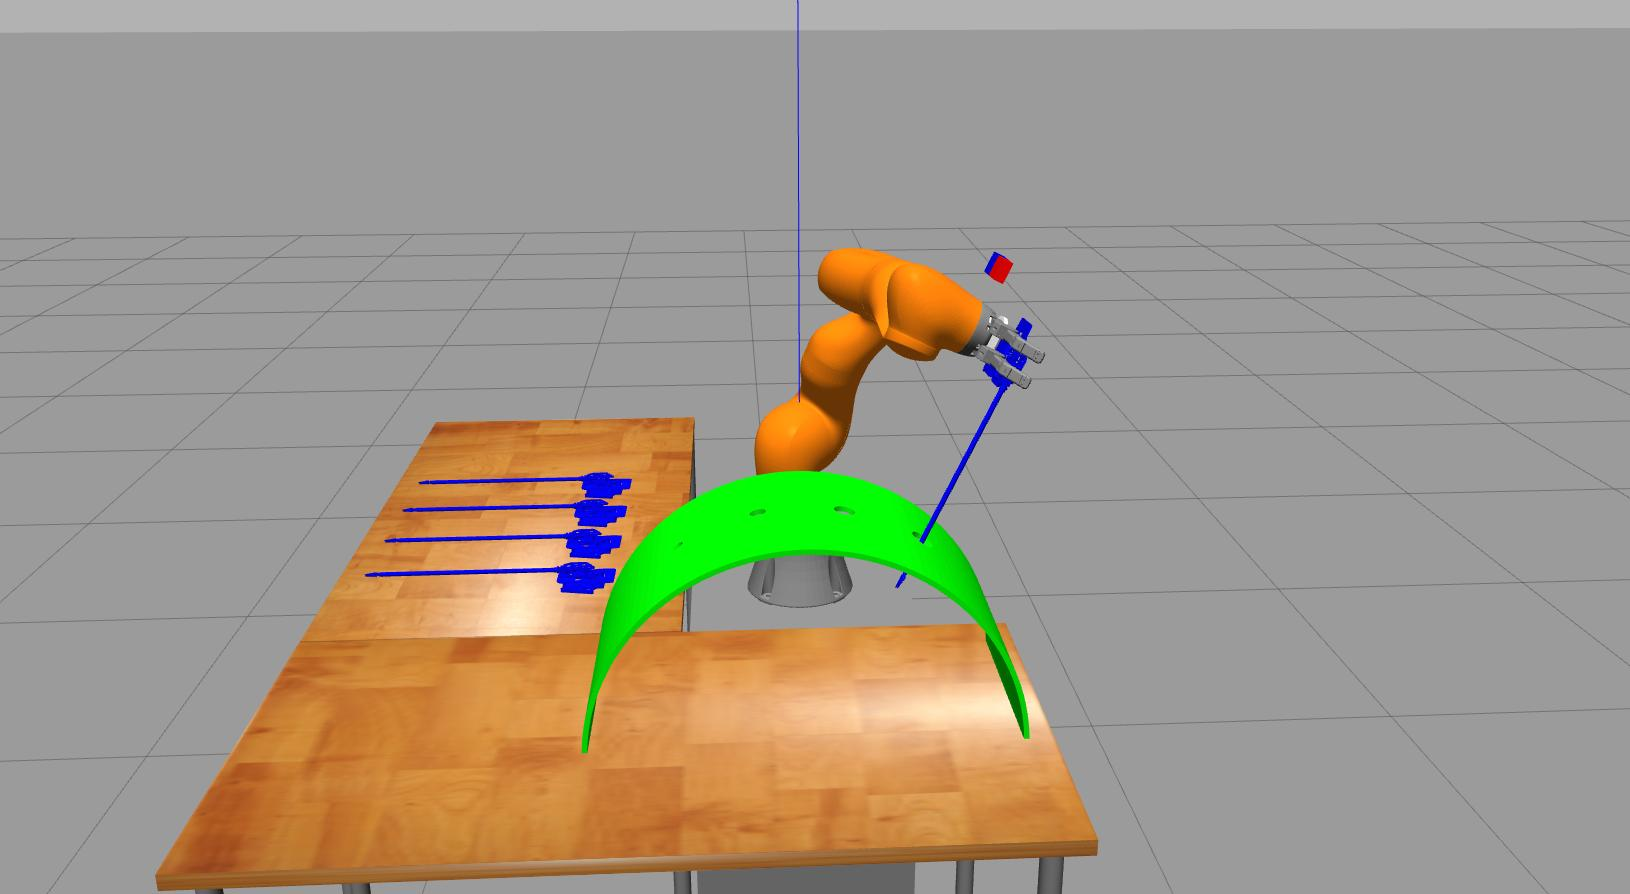
\includegraphics[width=0.3\textwidth]{images/robot_planner2b/robot_planner2b_2}
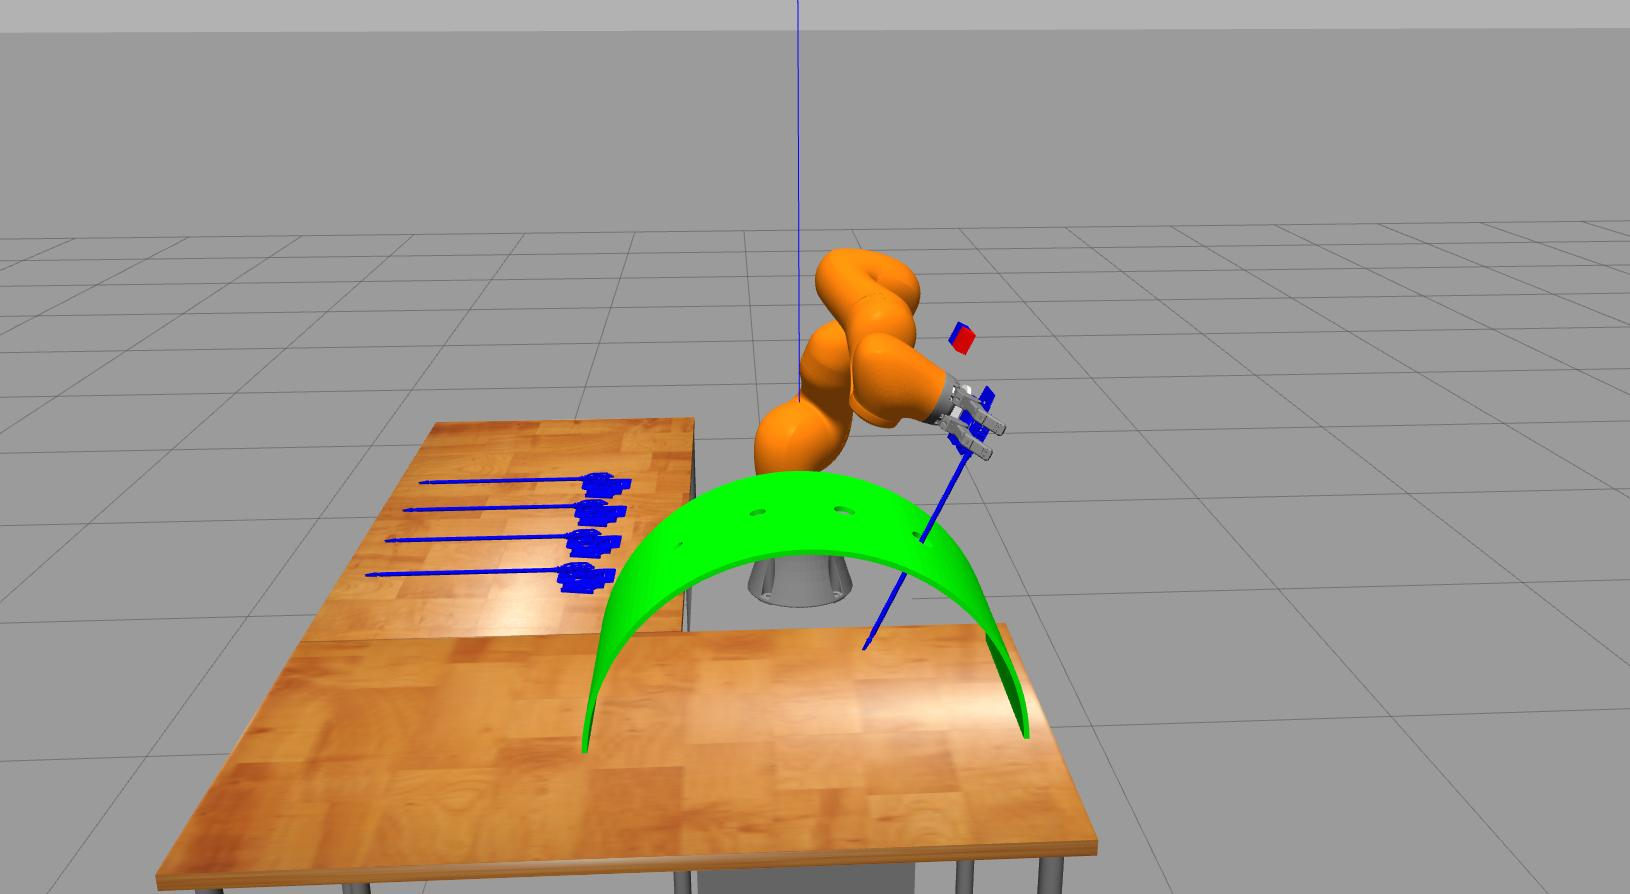
\includegraphics[width=0.3\textwidth]{images/robot_planner2b/robot_planner2b_3}\\
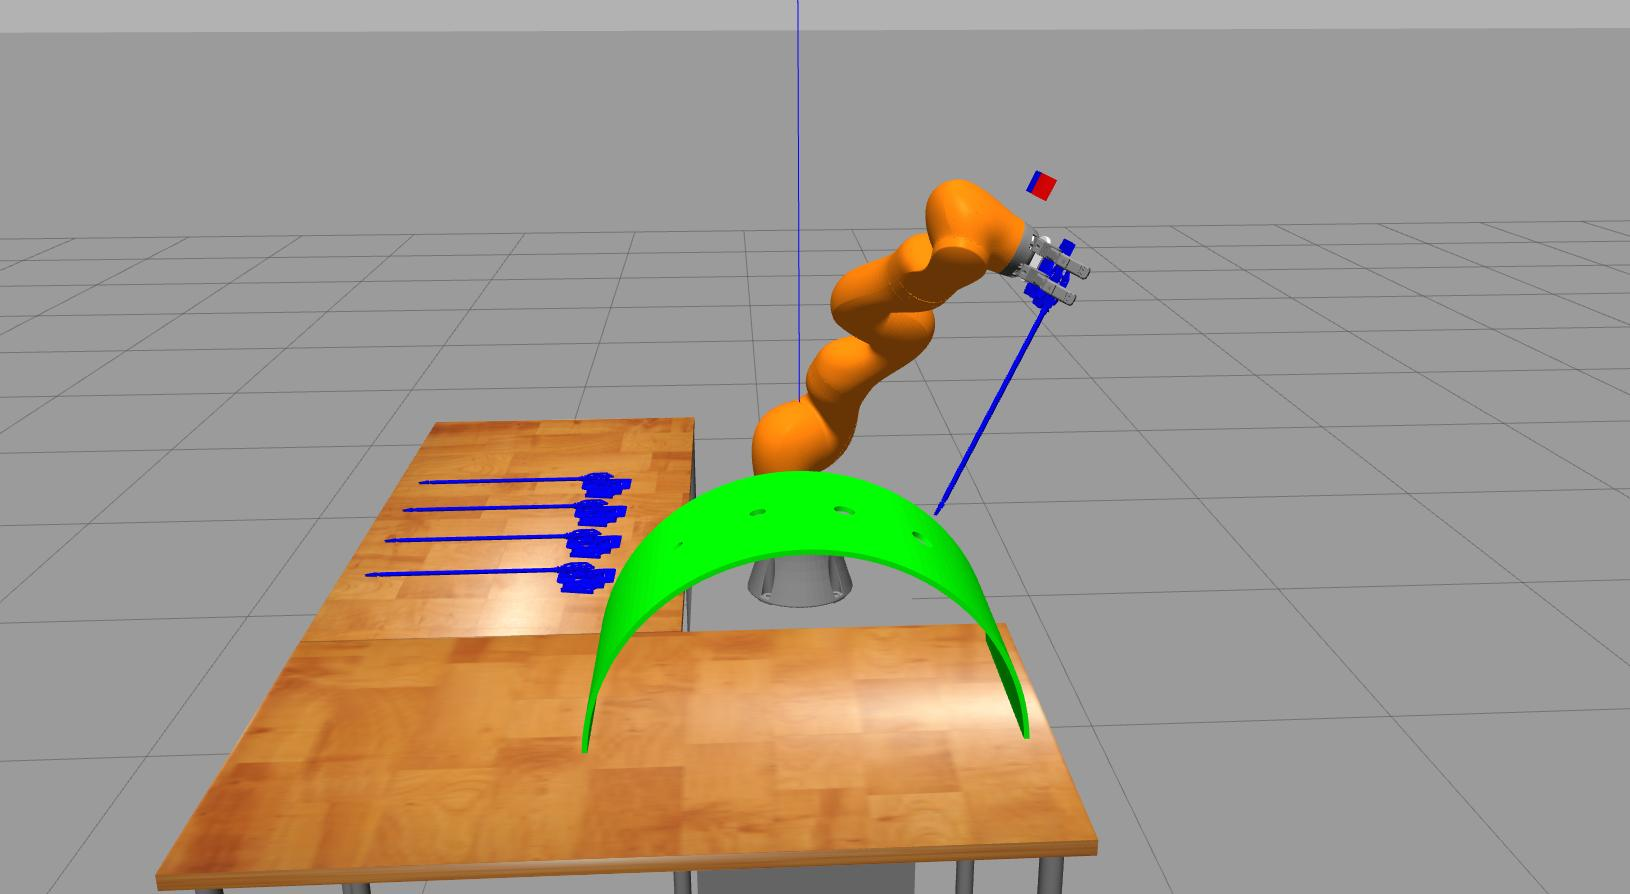
\includegraphics[width=0.3\textwidth]{images/robot_planner2b/robot_planner2b_4}
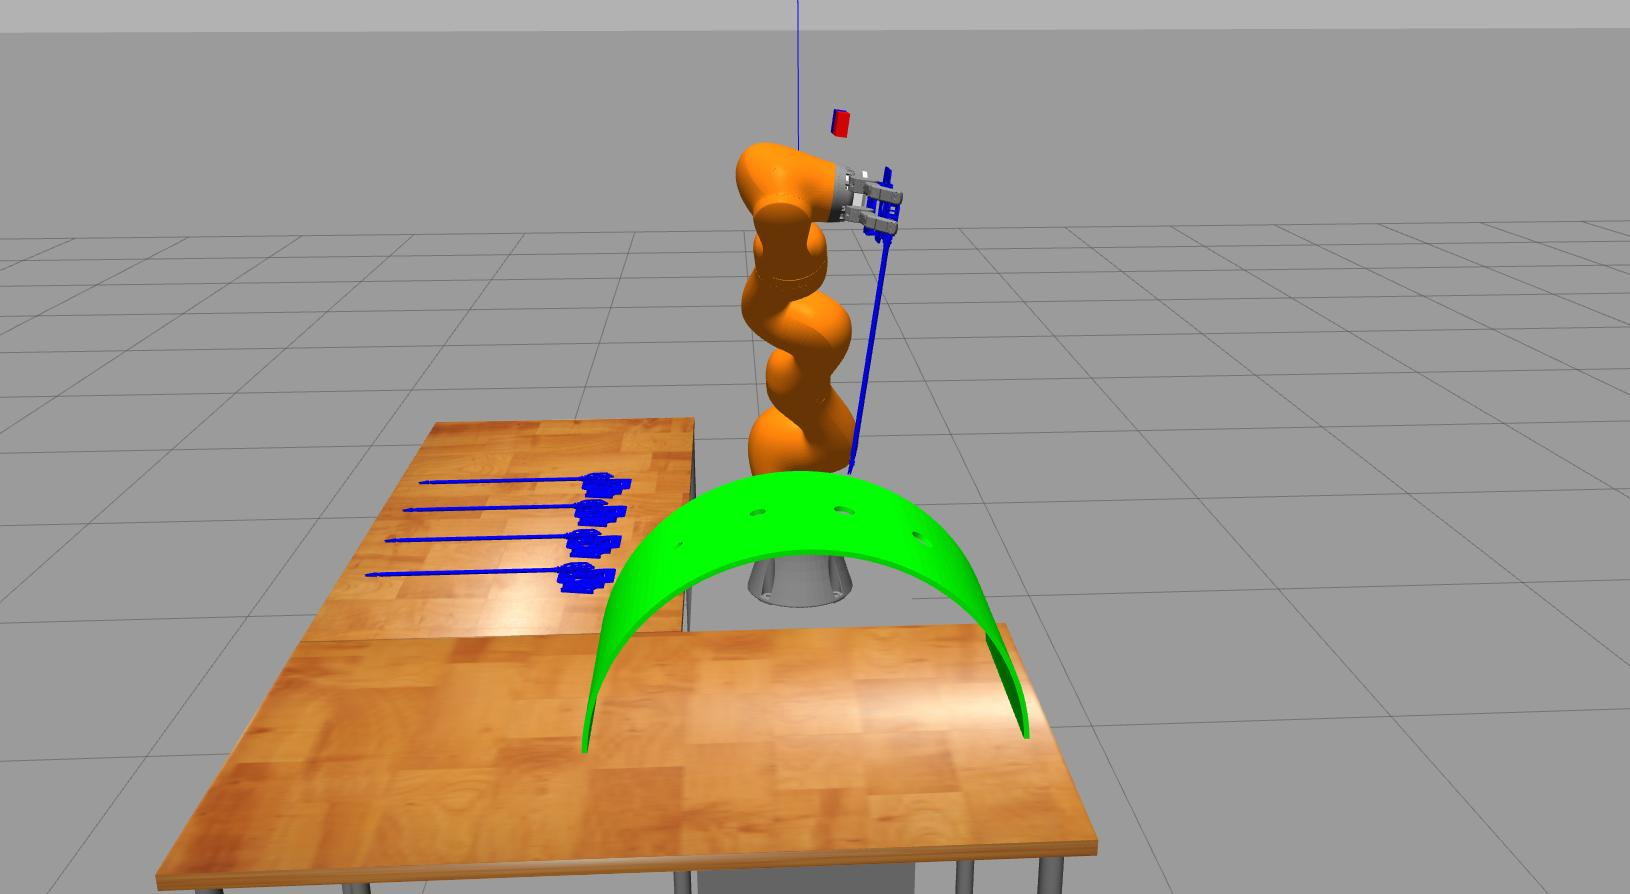
\includegraphics[width=0.3\textwidth]{images/robot_planner2b/robot_planner2b_5}
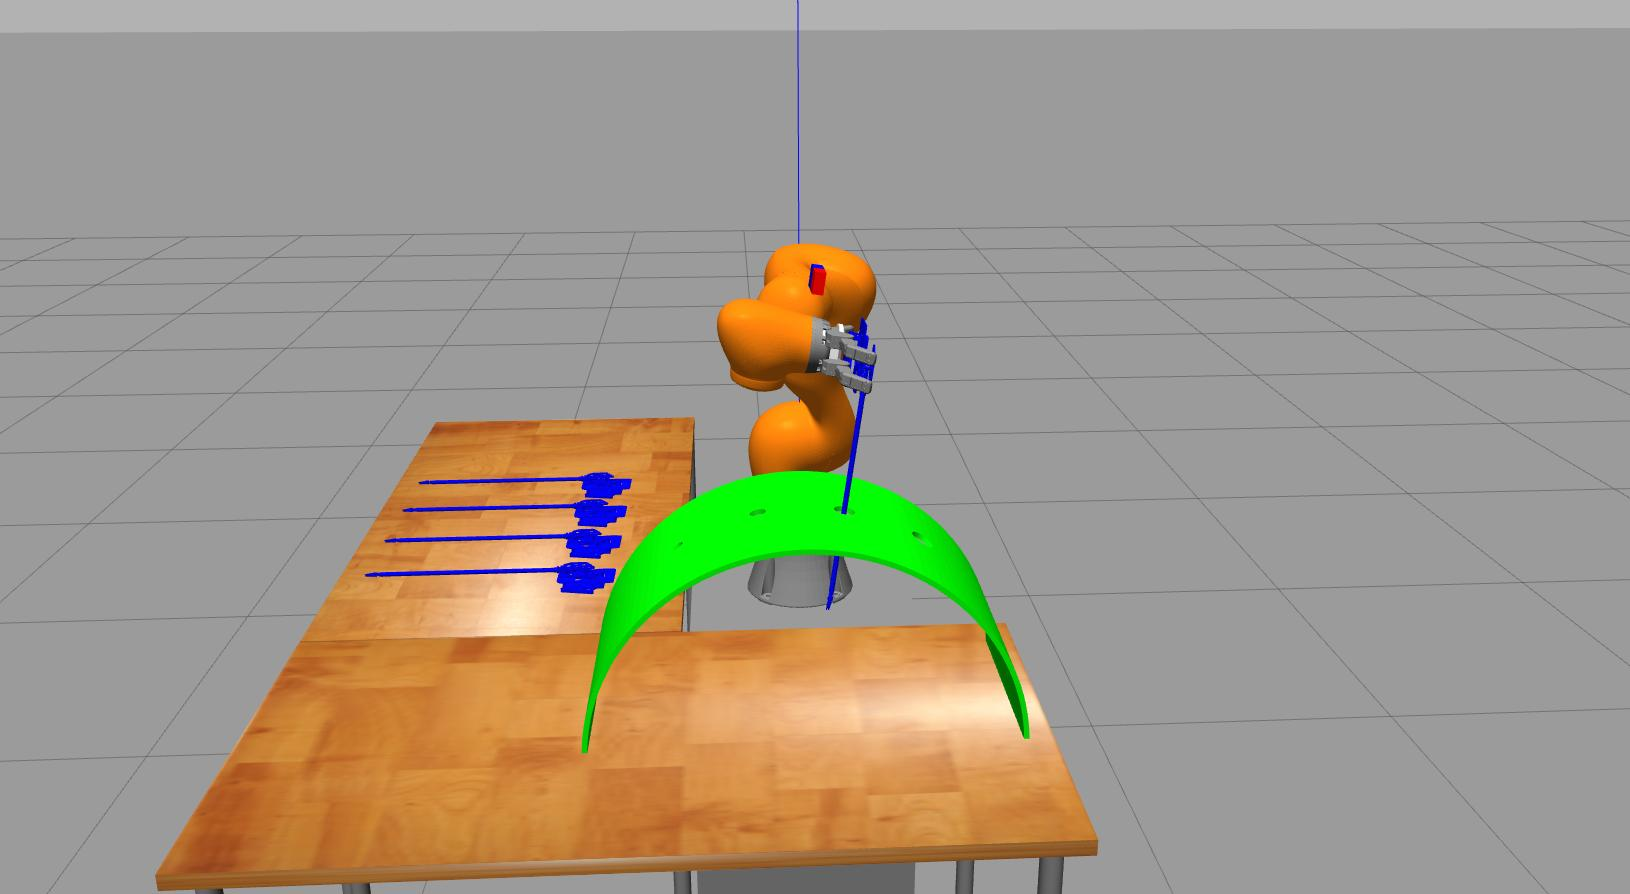
\includegraphics[width=0.3\textwidth]{images/robot_planner2b/robot_planner2b_6}\\
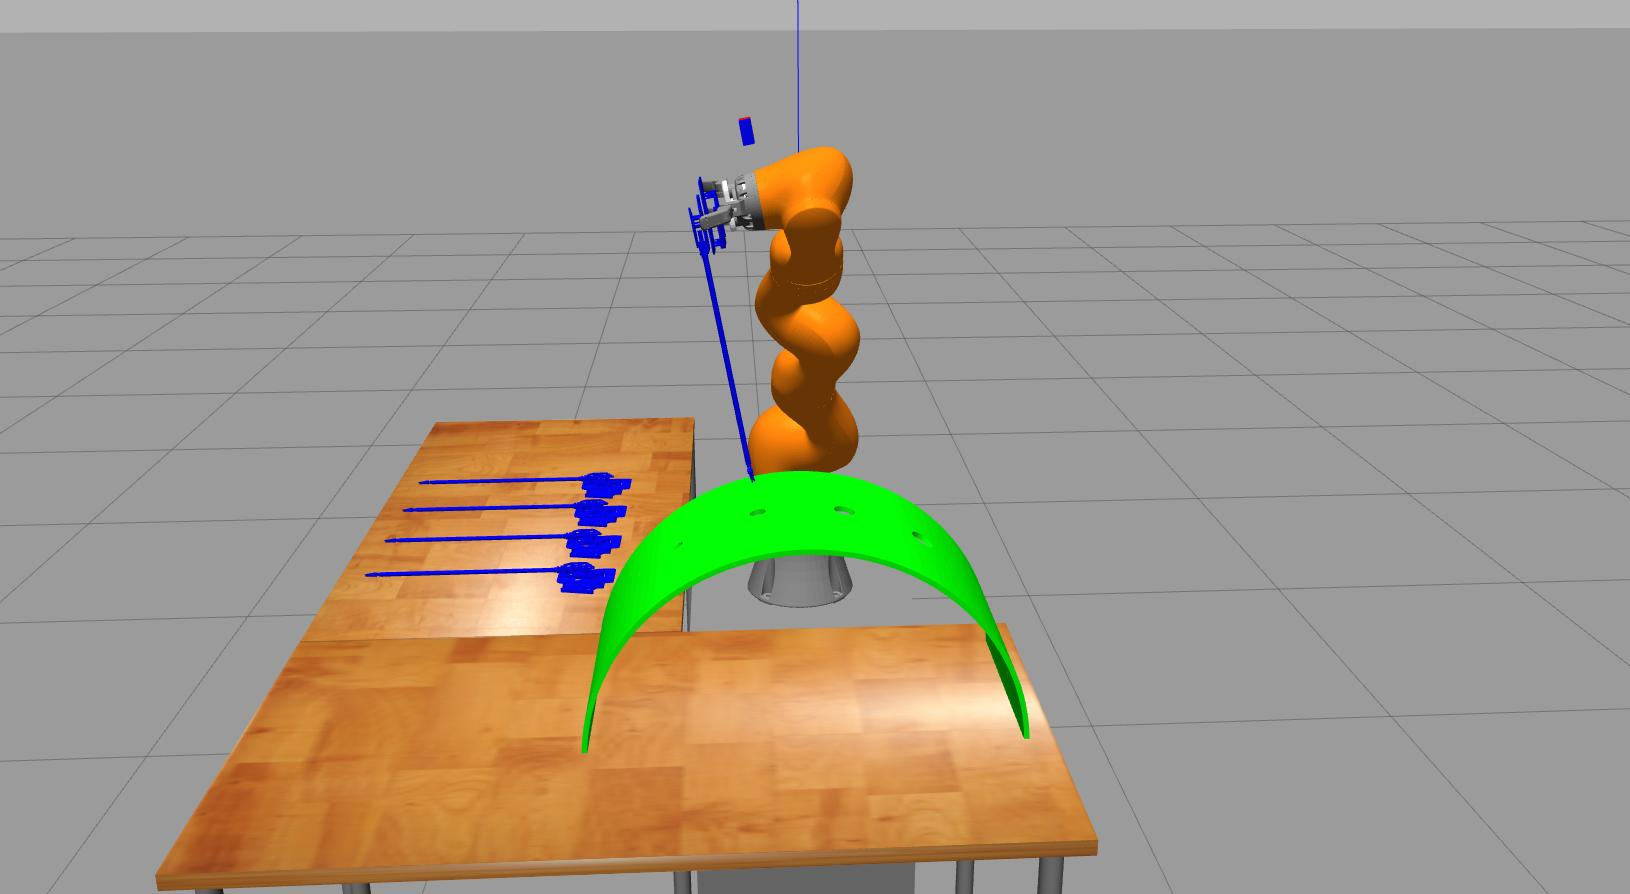
\includegraphics[width=0.3\textwidth]{images/robot_planner2b/robot_planner2b_7}
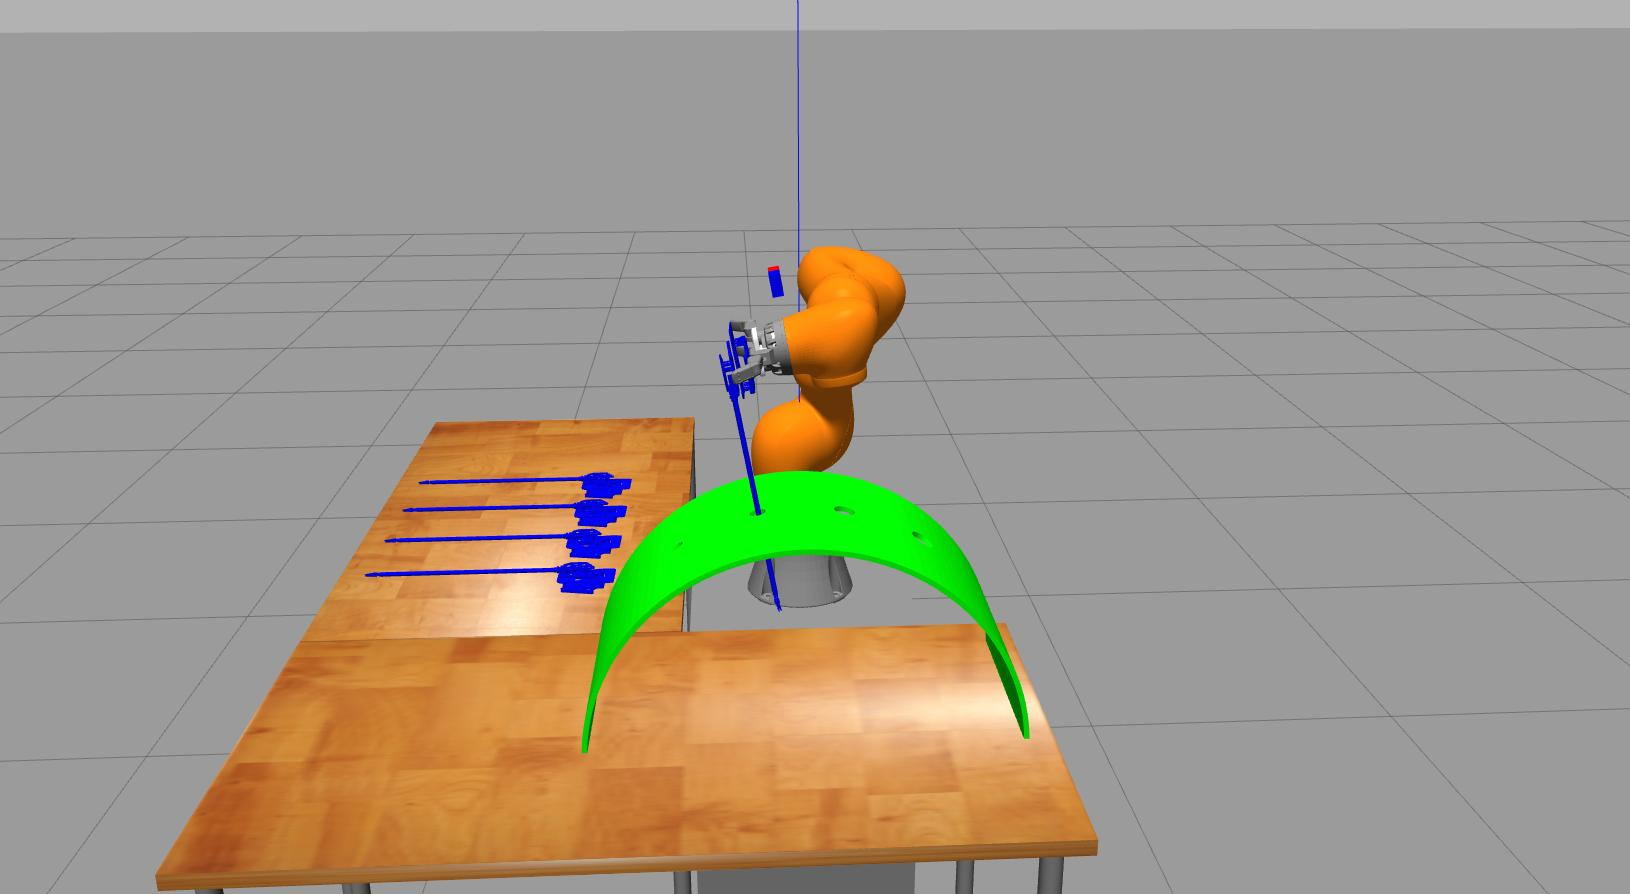
\includegraphics[width=0.3\textwidth]{images/robot_planner2b/robot_planner2b_8}
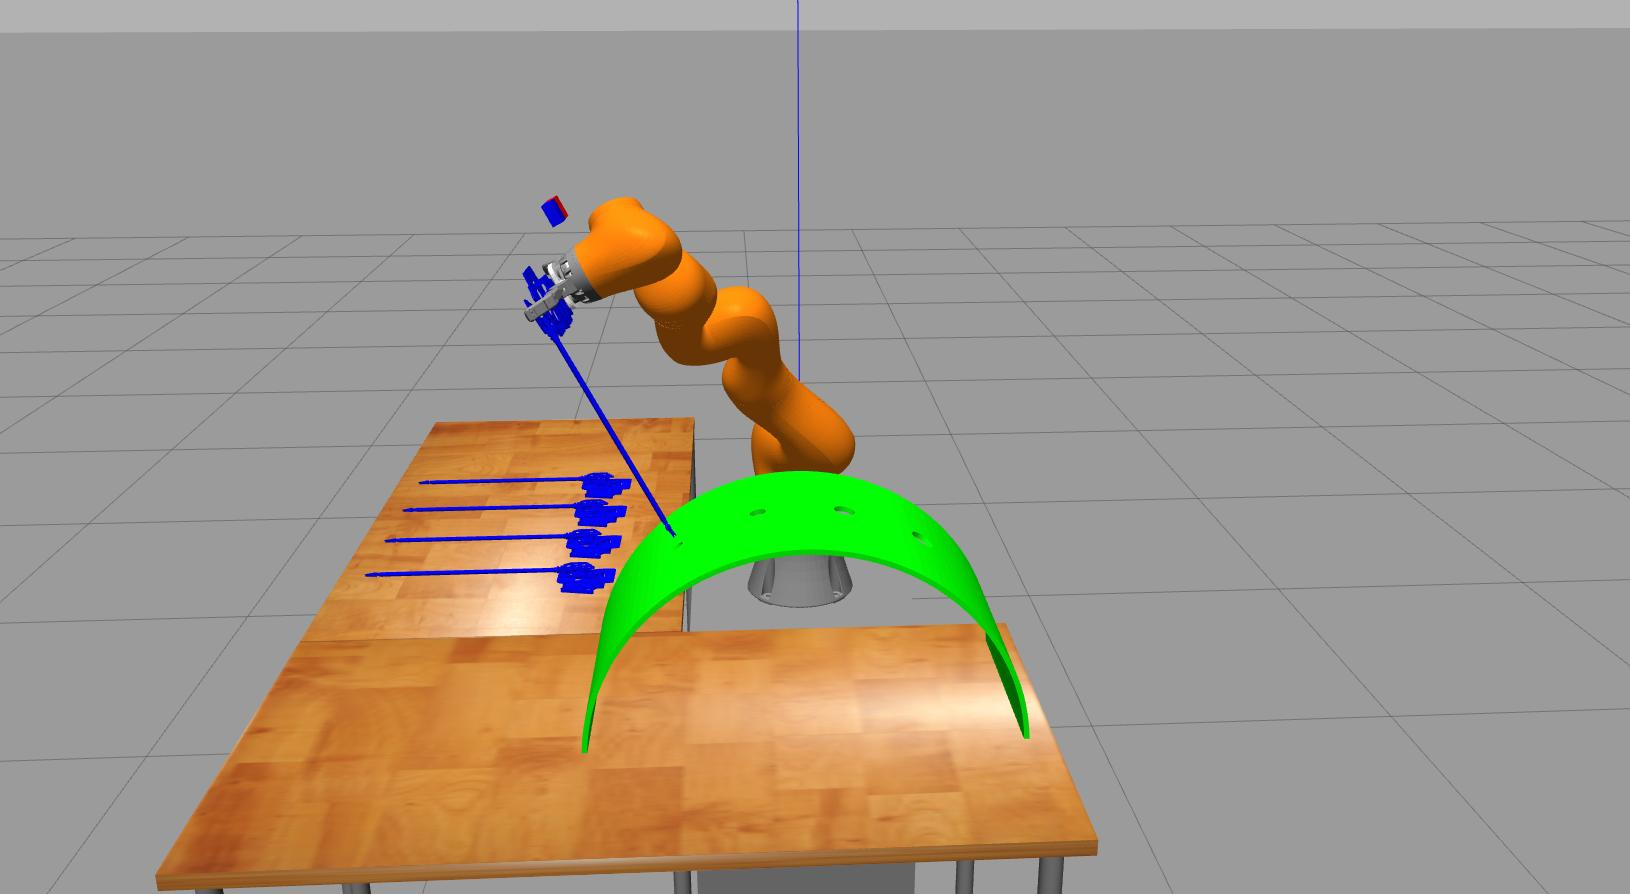
\includegraphics[width=0.3\textwidth]{images/robot_planner2b/robot_planner2b_9}\\
\caption{Experiment 2b:}
\end{figure}
\end{center}

Due to the probabilistic nature of the motion planner (in these experiments the OMPL library is used with the RRTConnect path planning algorithm), the solutions 
to the path planning problem are not always the same and thus it is possible that the robot arm reaches a pose which is close to a singularity
\begin{center}
\begin{figure}[H]
\centering
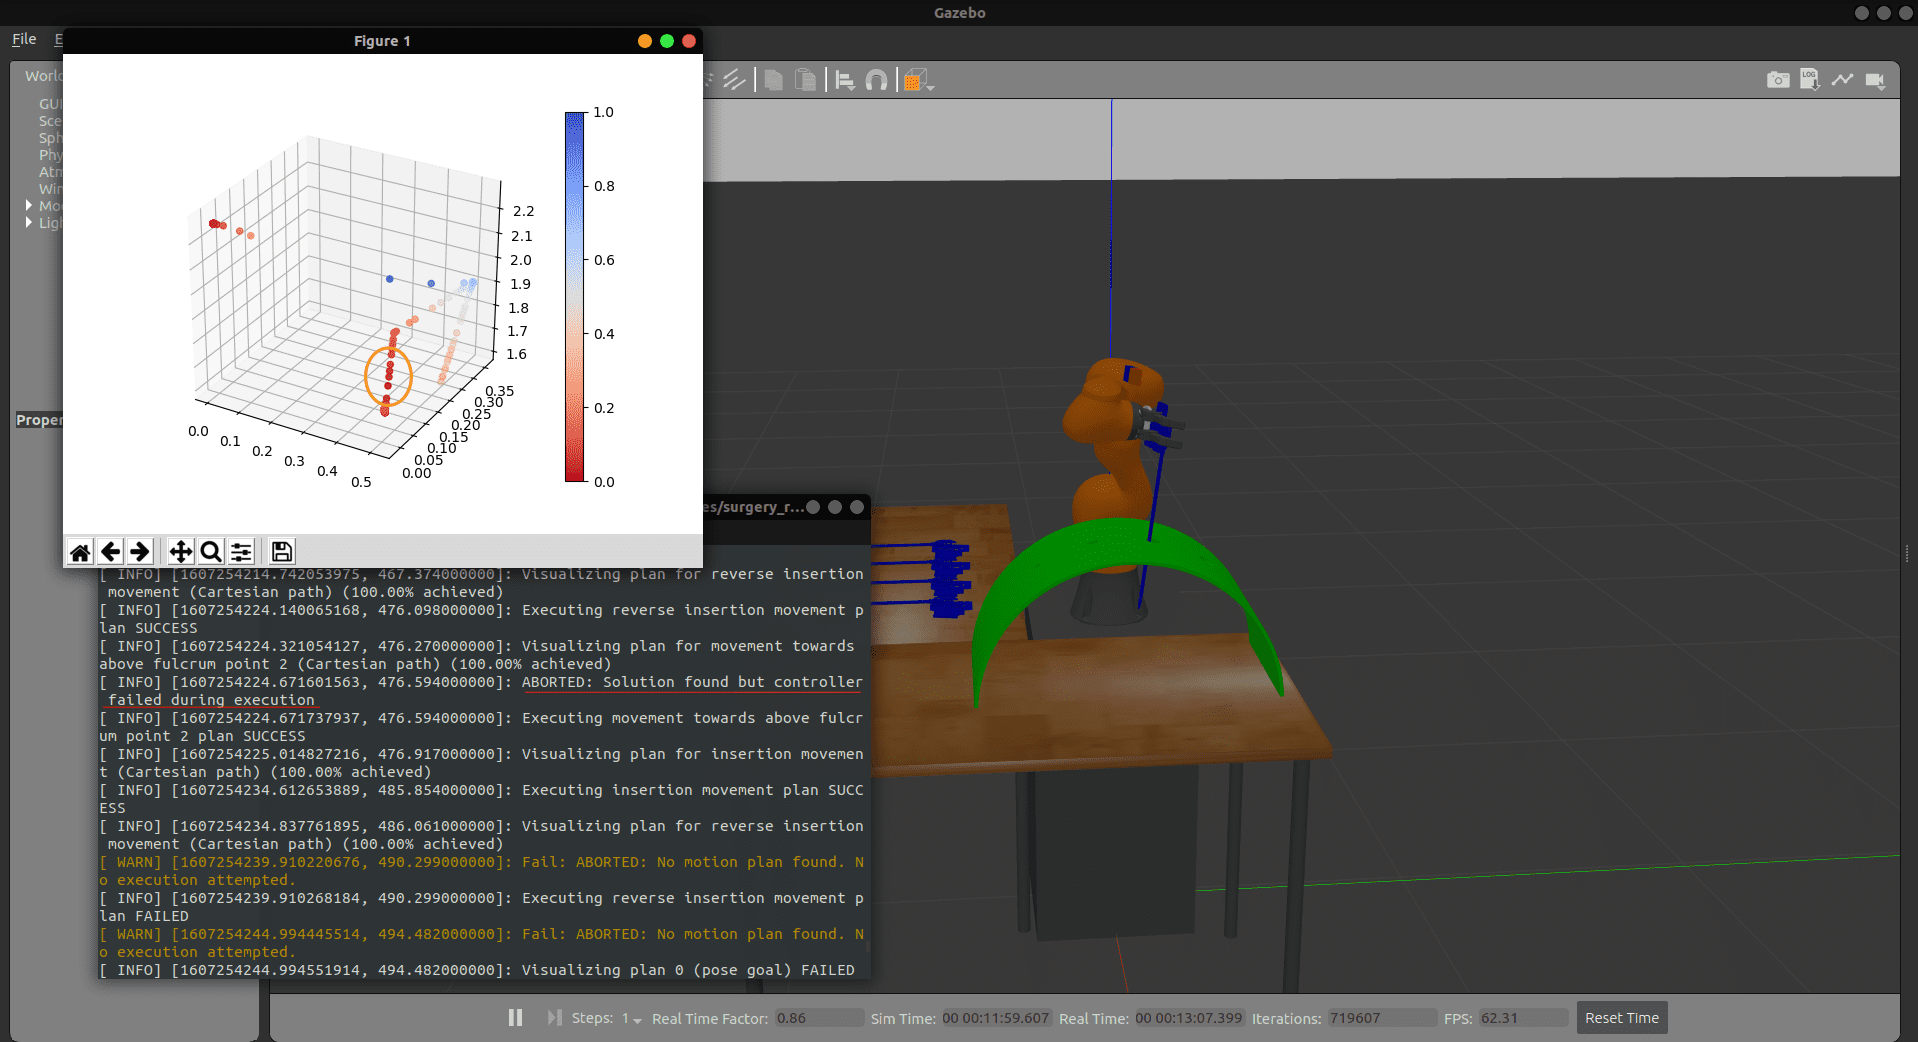
\includegraphics[width=0.9\textwidth]{images/robot_planner2b/singularity_failure.png}
\caption{Experiment 2b: Singularity failure}
\end{figure}
\end{center}

\subsubsection{Robot Planner 3}

\subsubsection{Robot Planner 4}

\subsubsection{Robot Planner 5}

